\documentclass[]{article}
\usepackage{amsmath, amsfonts}
\usepackage{graphicx, subcaption}
\usepackage{geometry}

\geometry{left=1in, right=1in, top=0.75in, bottom=0.75in}

% Title Page
\title{MA5678 Assignment}
\author{David Blair}

\newcommand{\real}{\mathbb{R}}
\def\incode#1{\texttt{#1}}

\begin{document}
	\vspace*{\fill}
	\begin{center}
		\includegraphics[scale = 0.15]{images/brunel logo.png}
		
		\vspace{1cm}
		\Large{Department of Mathematics, College of Engineering, Design and Physical Sciences, Brunel University}
		
		\vspace{1cm}
		\Large{MA5678: Numerical Methods}
		
		\vspace{1cm}
		\large{Academic Year 2022 - 2023}
		
		\vspace{1.5cm}
		\LARGE{\bf Assignment}
		
		\vspace{1cm}
		\large{By David Blair}
		
		\vspace{0.1cm}
		\large{Lecturer: Dr Jacques Furter}
	\end{center}
	\vspace*{\fill}
	\newpage
	\section{Stage 1: Logistic Growth Model}
	\subsection{Chosen Model}
	I have chosen to investigate the biological applications of numerical solutions to differential equations. I will be looking at the logistic equation: 
	
	\begin{align}
		\dot X(t) = rX(t)\left(1 - \frac{X(t)}{K}\right)	
		\label{eq:logistic_growth}	
	\end{align}
	
	Where $t \in [0, \infty)$ represents time and $X: [0, \infty) \rightarrow \mathbb{R}$. $r$ is the difference between the birth rate $b$ and the death rate $d$ where $r = b - d$. 
	$K$ represents the carrying capacity of the population. As $X(t)$ gets closer to $K$, $\dot X(t)$ decreases until it reaches 0 at $X(t) = K$.
	
	\subsection{Analytical Solution}
	We begin with our logistic equation, letting $X(t) = X$ and $\dot X(t) = \dot X$:
	
	\begin{align}
		\dot X = \frac{dX}{dt} = rX\left(1 - \frac{X}{K}\right)		
	\end{align}
	
	Firstly we separate the variables and integrate:
	
	\begin{align}
		\int\frac{1}{X\left(1 - \frac{X}{K}\right)} dX = \int r \hspace{2pt} dt
	\end{align}
	
	We can modify our integrand slightly:
	
	\begin{align}
		\frac{1}{X\left(1 - \frac{X}{K}\right)} = \frac{K}{X(K - X)} = \frac{1}{X} + \frac{1}{K - X}
	\end{align}
	
	Allowing us to determine the integral:
	
	\begin{align}
		\int\frac{1}{X\left(1 - \frac{X}{K}\right)} dX &= \int \frac{1}{X} dX + \int \frac{1}{K - X} dX \\
		&= ln|X| - ln|K - X| \\
		&= ln\left|\frac{X}{K - X}\right| = rt + C 
	\end{align}
	
	We can then rearrange the equation to get rid of the natural log:
	
	\begin{align}
		ln\left|\frac{K - X}{X}\right| &= -rt - C \\
		\frac{K - X}{X} &= e^{-rt - C} \\
		&= Ae^{-rt} \hspace{2pt} (A = \pm e^{-C})
	\end{align}
	
	If we set $t = 0$ and $X = X_0$ we can determine the value of $A$ as:
	
	\begin{align}
		A = \frac{K - X_0}{X_0}
	\end{align}
	
	Giving us the expression for $X(t)$:
	
	\begin{align}
		X(t) = \frac{K}{1 + Ae^{-rt}} \hspace{2pt} \text{where} \hspace{2pt} A = \frac{K - X_0}{X_0}
	\end{align}
	
	To plot this function, we first set $K = 100$ and $X_0 = 10$. We then take different growth rates with some being negative and some positive 
	in order to observe different behaviour:
	
	\begin{figure}[h]
		\centering
		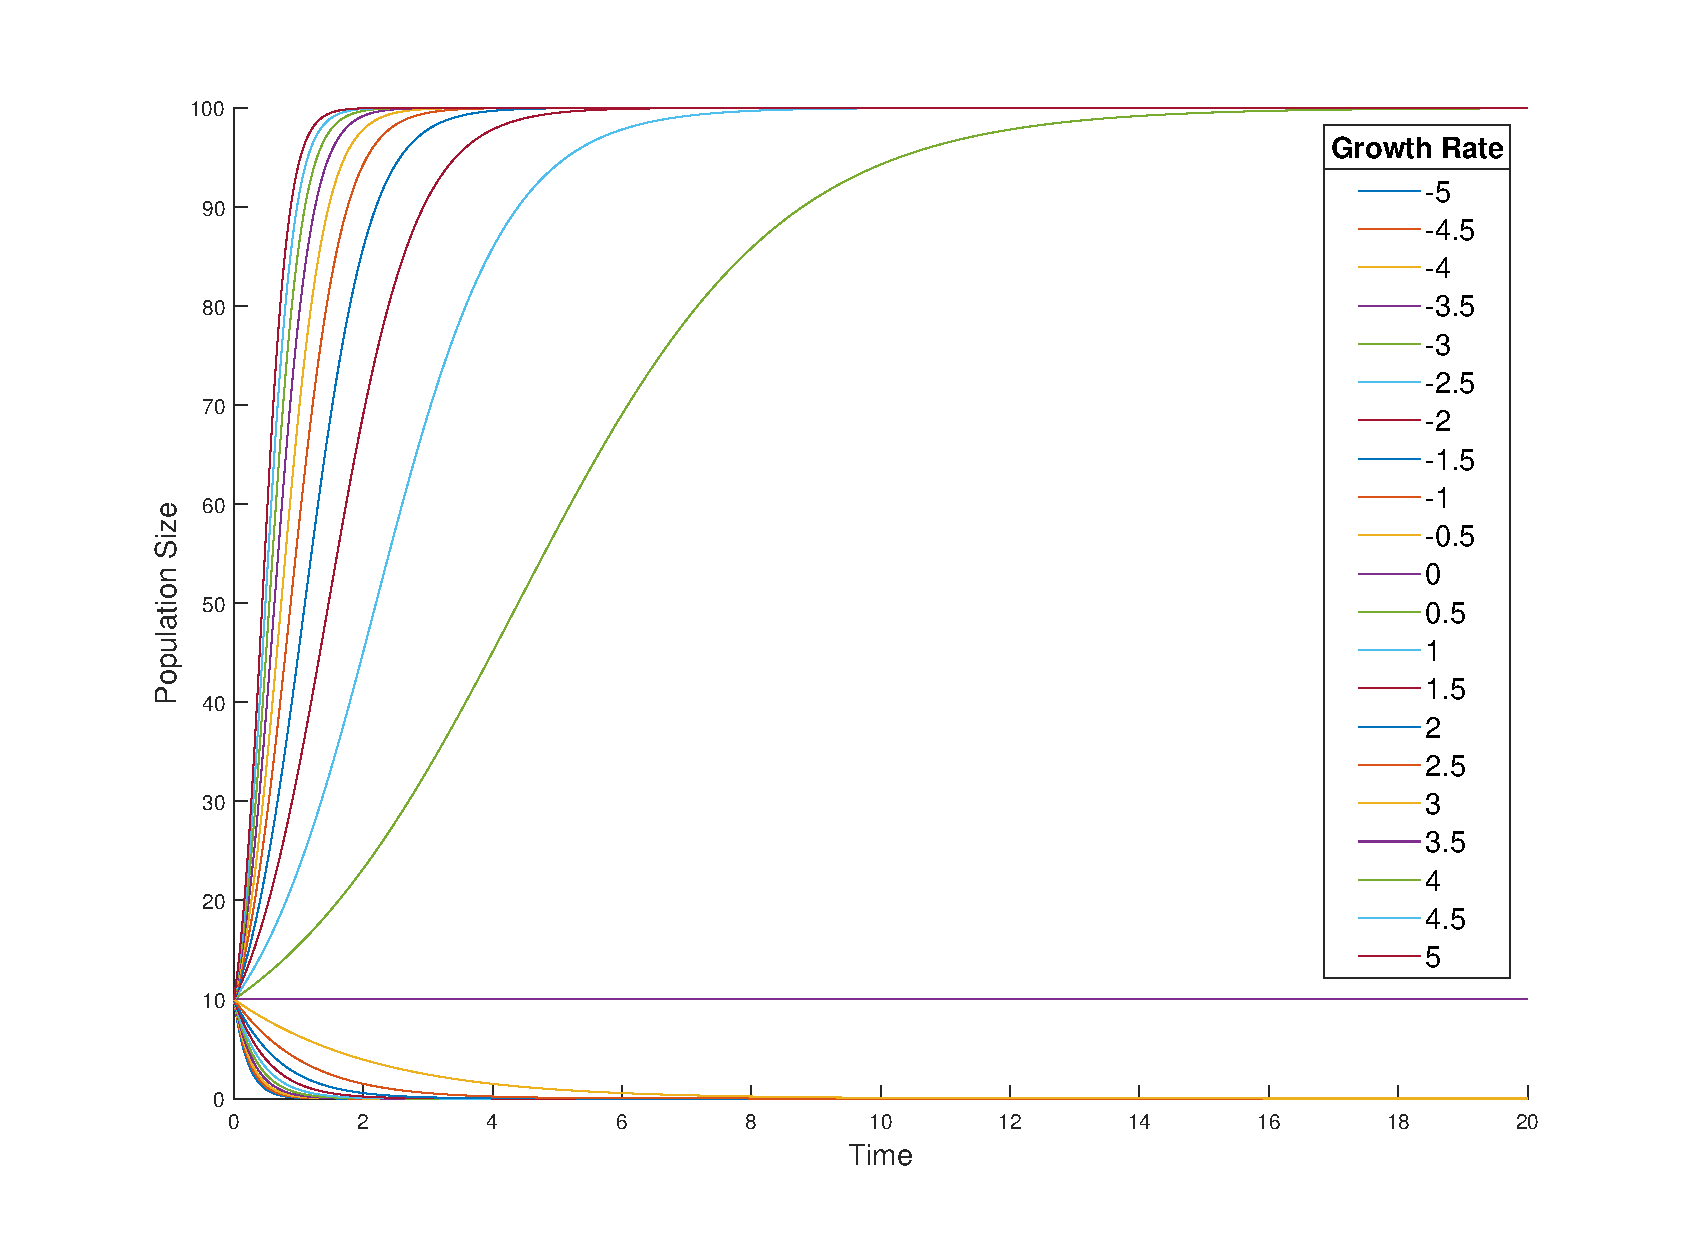
\includegraphics[scale = 0.35]{images/logistic_model.eps}
		\caption{Logistic Models with Varying Growth Rates}
		\label{fig:logistic_model}
	\end{figure}

	The code to produce figure \ref{fig:logistic_model} can be found in \incode{logistic\_model.m}.
	
	When the growth rate is 0, the population doesn't change. A negative growth rate will force the population to tend towards 0 and those 
	rates with a higher magnitude will reach 0 faster. Similarly, a positive growth rate will lead to an exponential growth in the population 
	before it slows down as it reaches the carrying capacity. A rate with a higher magnitude will induce a much faster exponential growth before it 
	reaches the carrying capacity.
	
	\subsection{Logistic Stochastic ODE}
	The logistic equation given in equation \ref{eq:logistic_growth} has an equivalent logistic stochastic ODE:
	
	\begin{align}
		dX = rX(t)\left(1 - \frac{X(t)}{K}\right)dt + \sigma X(t)dW
		\label{eq:logistic_stochastic}
	\end{align} 
	
	Where $X(t)$ is the population, $r$ is the intrinsic growth, $\sigma$ is the volatility and $dW$ is a Wiener process (the probabilistic element of equation \ref{eq:logistic_stochastic}). The complexity of the solution to this ODE means that we will be using a simpler approximation to run our simulations: 
	
	\begin{align}
		X_k - X_{k - 1} = rX_{k - 1}\left(1 - \frac{X_{k - 1}}{K}\right)\Delta t + \sigma X_{k - 1}\epsilon (k - 1)\sqrt{\Delta t}, \hspace{2pt} 1 \leq k \leq N
	\end{align}
	
	Where $\Delta t$ is the discrete time-step, $\epsilon (k - 1) \in \mathcal{N}(0, 1)$ is a random number drawn at every time step and $\sigma$ is the volatility. The initial value of the population is $S_0$. $N$ is the number of steps of the simulation. $N \Delta t = T$ where $T$ is the time horizon of the run. 
	
	To run this function, we set $N = 90$, $X_0 = 30$, $K = 20$ and $r = 0.05$. The volatility $\sigma \in \{-0.2, -0.1, 0, 0.1, 0.2\}$ and the time horizon $T \in \{80, 120\}$. See figure \ref{fig:stochastic_model}.
	
	\begin{figure}[h!]
		\centering
		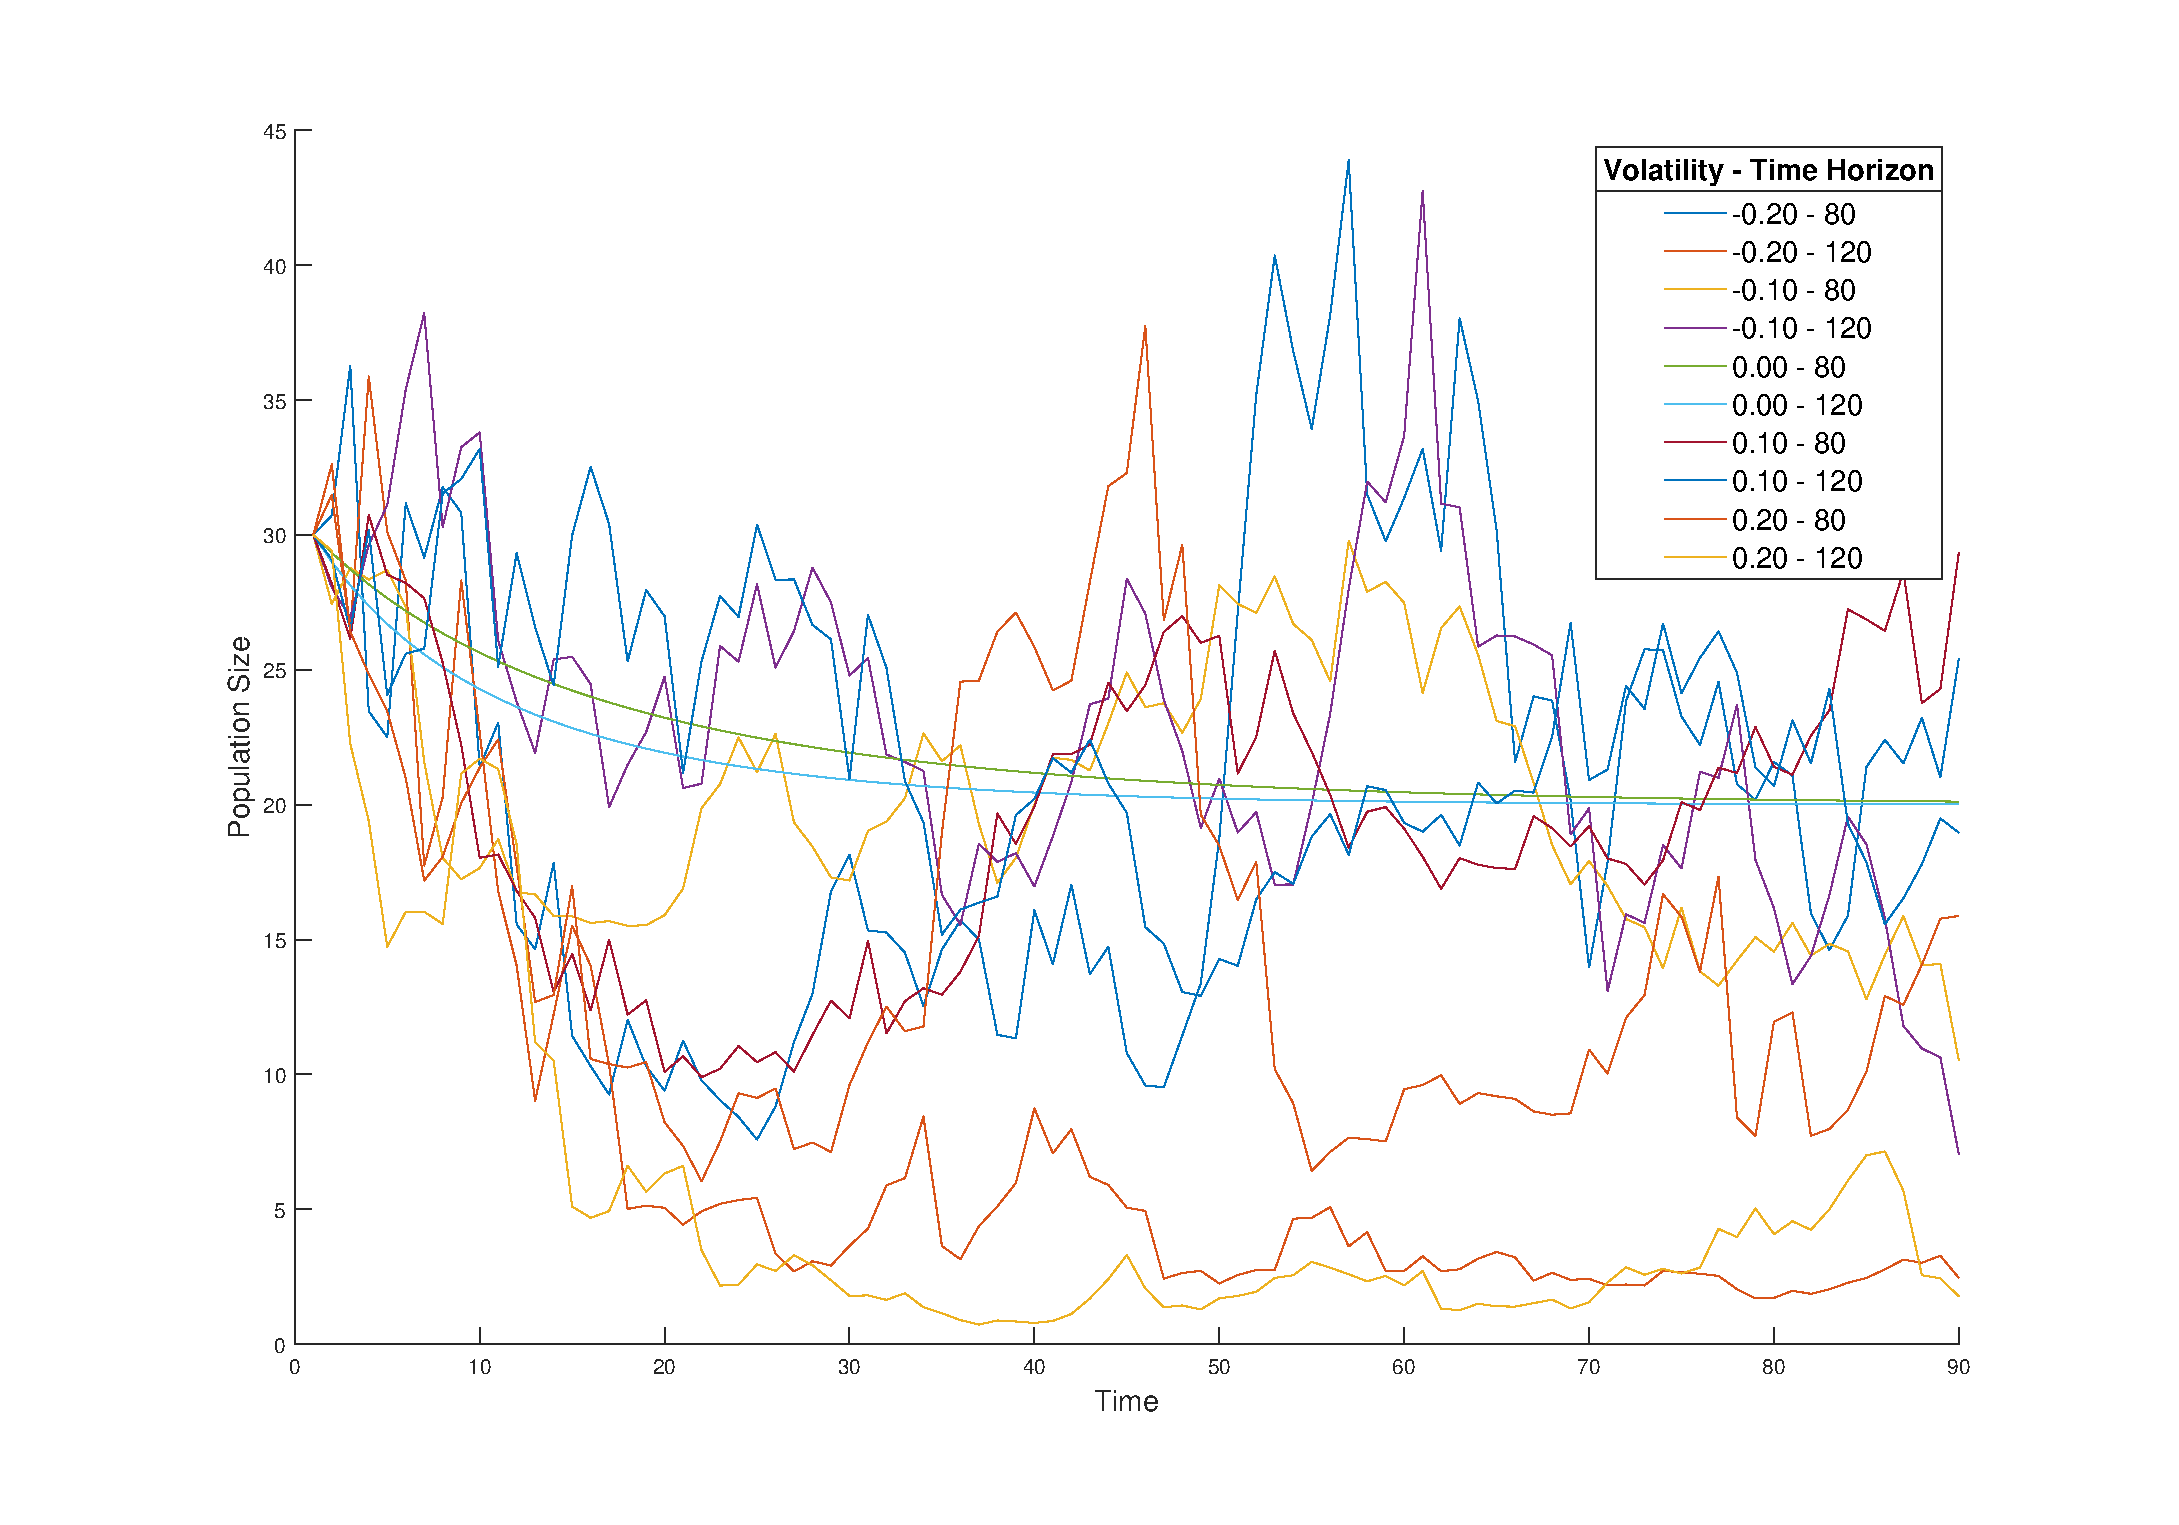
\includegraphics[scale=0.29]{images/stochastic_model.eps}
		\caption{Stochastic Model at Different Values of $T$ and $\sigma$}
		\label{fig:stochastic_model}
	\end{figure}

	The code to produce figure \ref{fig:stochastic_model} can be found in \incode{stochastic\_model.m}.
	
	When we set $\sigma = 0$, it is clear that a lower time horizon results in a shallower curve which has no fluctuation. A higher magnitude in the volatility results in greater fluctuations around the initial value line.
	
	Each time we run the simulation, we are using a random number generator to sample from a normal distribution. Because of this, its slightly harder to extract meaningful information as to the effect of varying our volatility and time horizon. If we ensure that the seed we use to generate these random numbers stays the same across simulations, the random numbers selected at each step become constants and we get some interesting results:
	
	\begin{figure}[h!]
		\centering
		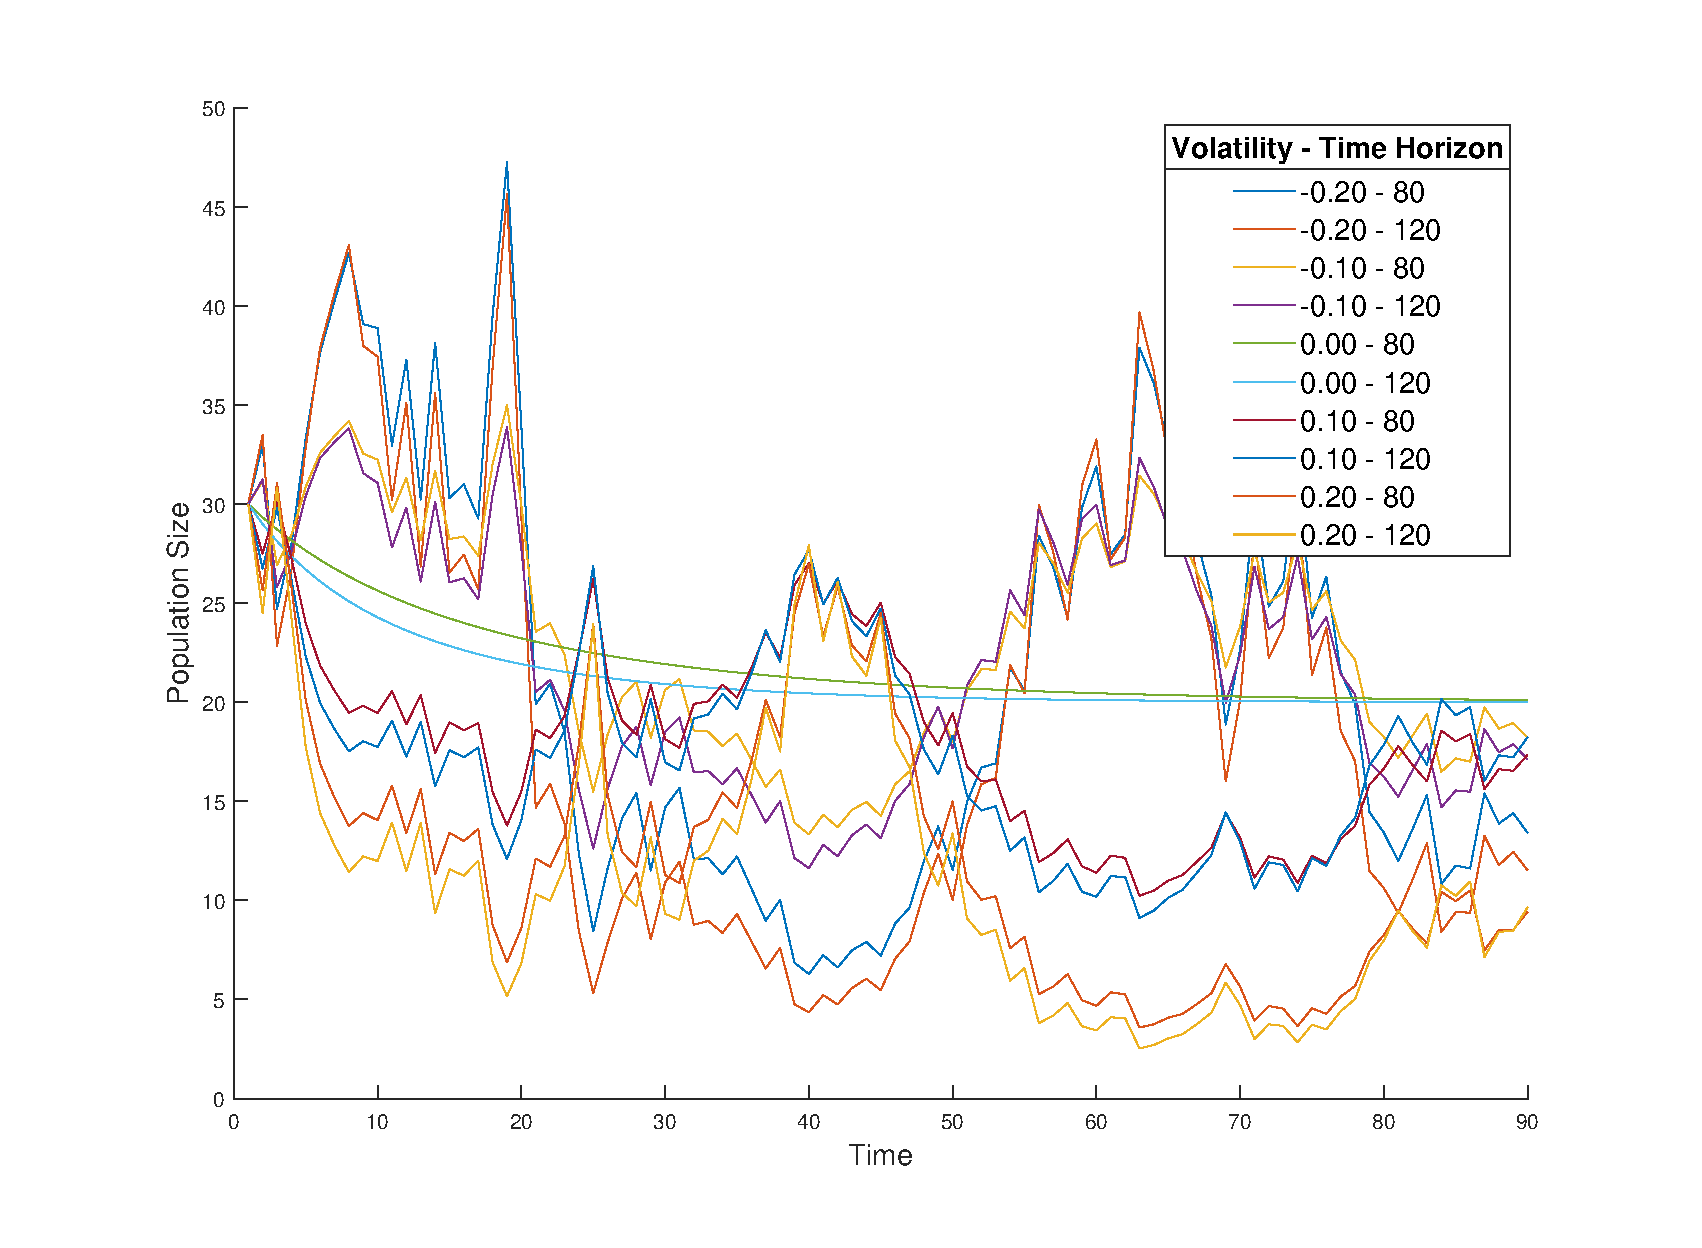
\includegraphics[scale=0.35]{images/stochastic_model_const.eps}
		\caption{Stochastic Model at Different Values of $T$ and $\sigma$ with Constant Seed Across Runs}
	\end{figure}
	
	\section{Stage 2}
	\subsection{Advection (Transport) Equation}
	The advection equation is as follows:
	\begin{align}
		\frac{\partial u}{\partial t} + c \frac{\partial u}{\partial x} = 0
	\end{align}
	Defined on the domain $ \real \times [0, \infty] $ with initial condition $ u(x, 0) = f(x) $. A solution to this equation is $ u(x, t) = f(x - ct) $:
	\begin{align}
		\frac{\partial u(x, t)}{\partial t} = \frac{\partial f(x - ct)}{\partial t} = -c f^\prime(x - ct) \nonumber \\
		\frac{\partial u(x, t)}{\partial x} = \frac{\partial f(x - ct)}{\partial x} = f^\prime(x - ct) \nonumber \\ \nonumber \\
		-c f^\prime(x - ct) + cf^\prime(x - ct) = 0 \nonumber \\ \nonumber \\ \nonumber 
		u(x, 0) = f(x - (0)t) = f(x)
	\end{align}

	To alter this differential equation so that we can solve it numerically, we start with the advection equation and rearrange:
	\begin{align}
		\frac{\partial u}{\partial t} + c \frac{\partial u}{\partial x} = 0 \\
		\frac{\partial u}{\partial t} =  -c \frac{\partial u}{\partial x} 
	\end{align}
	We then discretise the partial derivatives. Let $u(i, j)$ be the numerical approximation to $u$ at the $i$-th spacial point and the $j$-th time step. The left-hand side can be approximated by the forward difference in time and the right-hand side can be approximated using the backwards difference in space. This gives the following equation:
	\begin{align}
		\frac{u(i, j + 1) - u(i, j)}{\Delta t} = -c \frac{u(i, j) - u(i - 1, j)}{\Delta x}
	\end{align}
	Finally, we rearrange to give the updated formula: 
	\begin{align}
		u(i, j + 1) = u(i, j) - c\frac{\Delta t}{\Delta x}(u(i, j) - u(i - 1, j))
	\end{align}

	\noindent In \incode{transport.m}, you can find the code to solve this equation numerically. The algorithm is as follows:
	\begin{enumerate}
		\item We define a number of values based on the given parameters:
		\begin{enumerate}
			\item \incode{N}: The number of spacial grid points.
			\item \incode{xmax}: Redefined upper bound for the $x$ axis, based on the value of \incode{N}.
			\item \incode{M}: The number of temporal grid points. 
			\item \incode{k1} and \incode{k2}: Coefficients that simplify the discretised solution equation.
			\item \incode{solutions}: An array to hold the solutions (all values initialised as zero). 
			\item \incode{vetx}: An array holding the spacial grid point values.
		\end{enumerate}
		\item Secondly, we initialise the \incode{solutions} array with the starting conditions.
		\item Lastly, for each column of temporal grid points, we evaluate the solution at the next spacial grid point based on the previous value. This gives us a final array containing our solutions.
	\end{enumerate}
	To run this function, you can execute the code in the file \incode{main\_transport.m}. You can change the function you want to use for initialisation by amending the final parameter \incode{f0}. The values we used are as follow: \incode{xmin} $= 0$, \incode{dx} $= 0.01$, \incode{xmax} $= 10$, \incode{dt} $= 0.01$, \incode{tmax} $= 10$, \incode{c} $= 1$ and \incode{f0} $= x^2$. 
	
	In order to plot the results, we have modified the \incode{TransportPlot.m} function. Instead of plotting 4 different cross-sectional plots, it plots a 3D graph to illustrate all the data on one plot. You can see this by running the file \incode{main\_TransportPlot.m}. Below you'll find some plots for various functions:
	
	\begin{figure}[htbp]
		\centering
		\begin{subfigure}[b]{0.45\textwidth}
			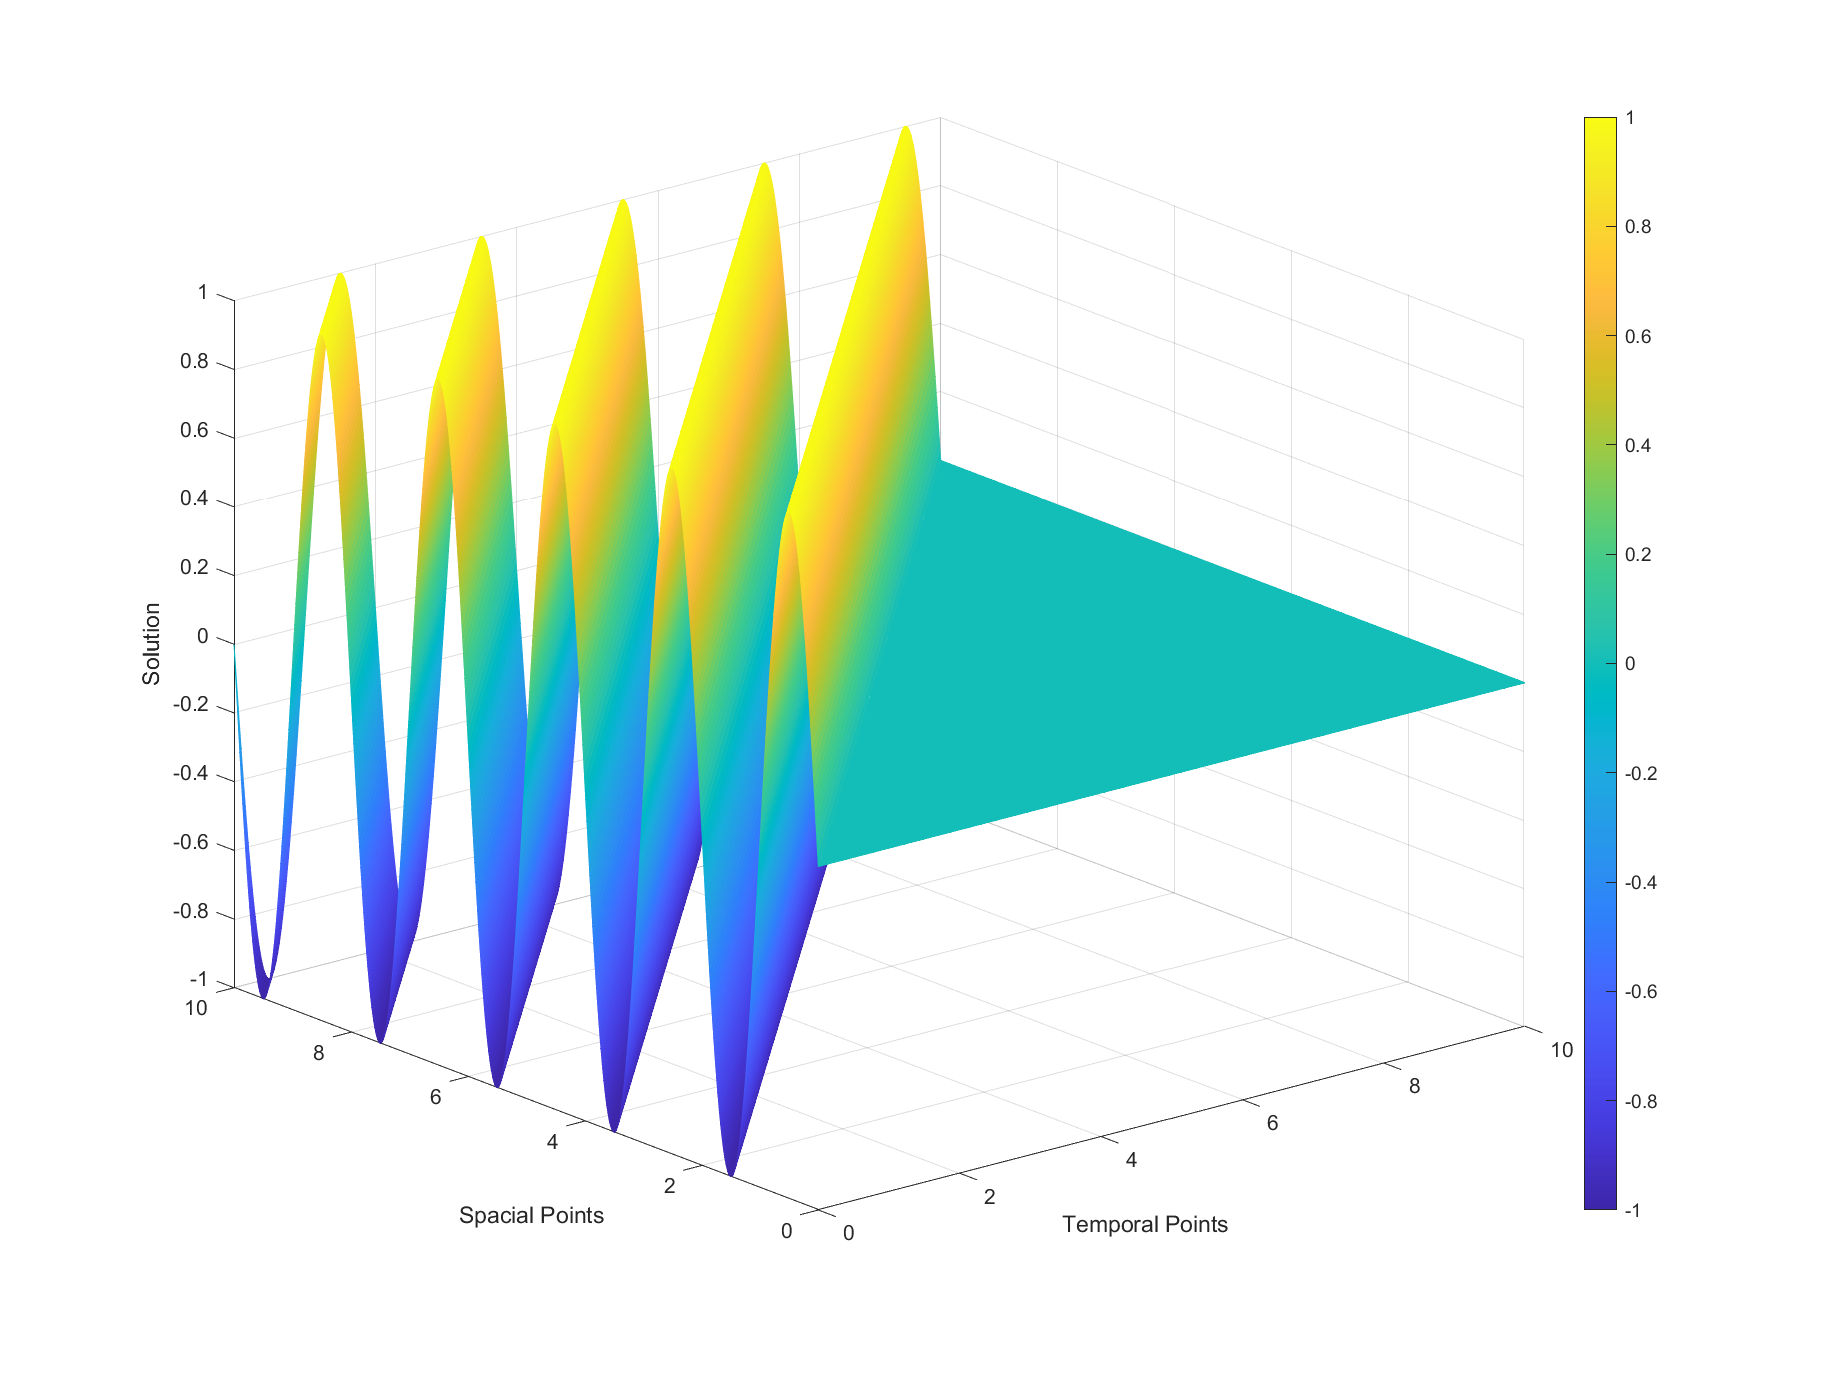
\includegraphics[width=\textwidth]{images/f0_side.eps}
			\caption{Side View}
		\end{subfigure}
		\hfill
		\begin{subfigure}[b]{0.45\textwidth}
			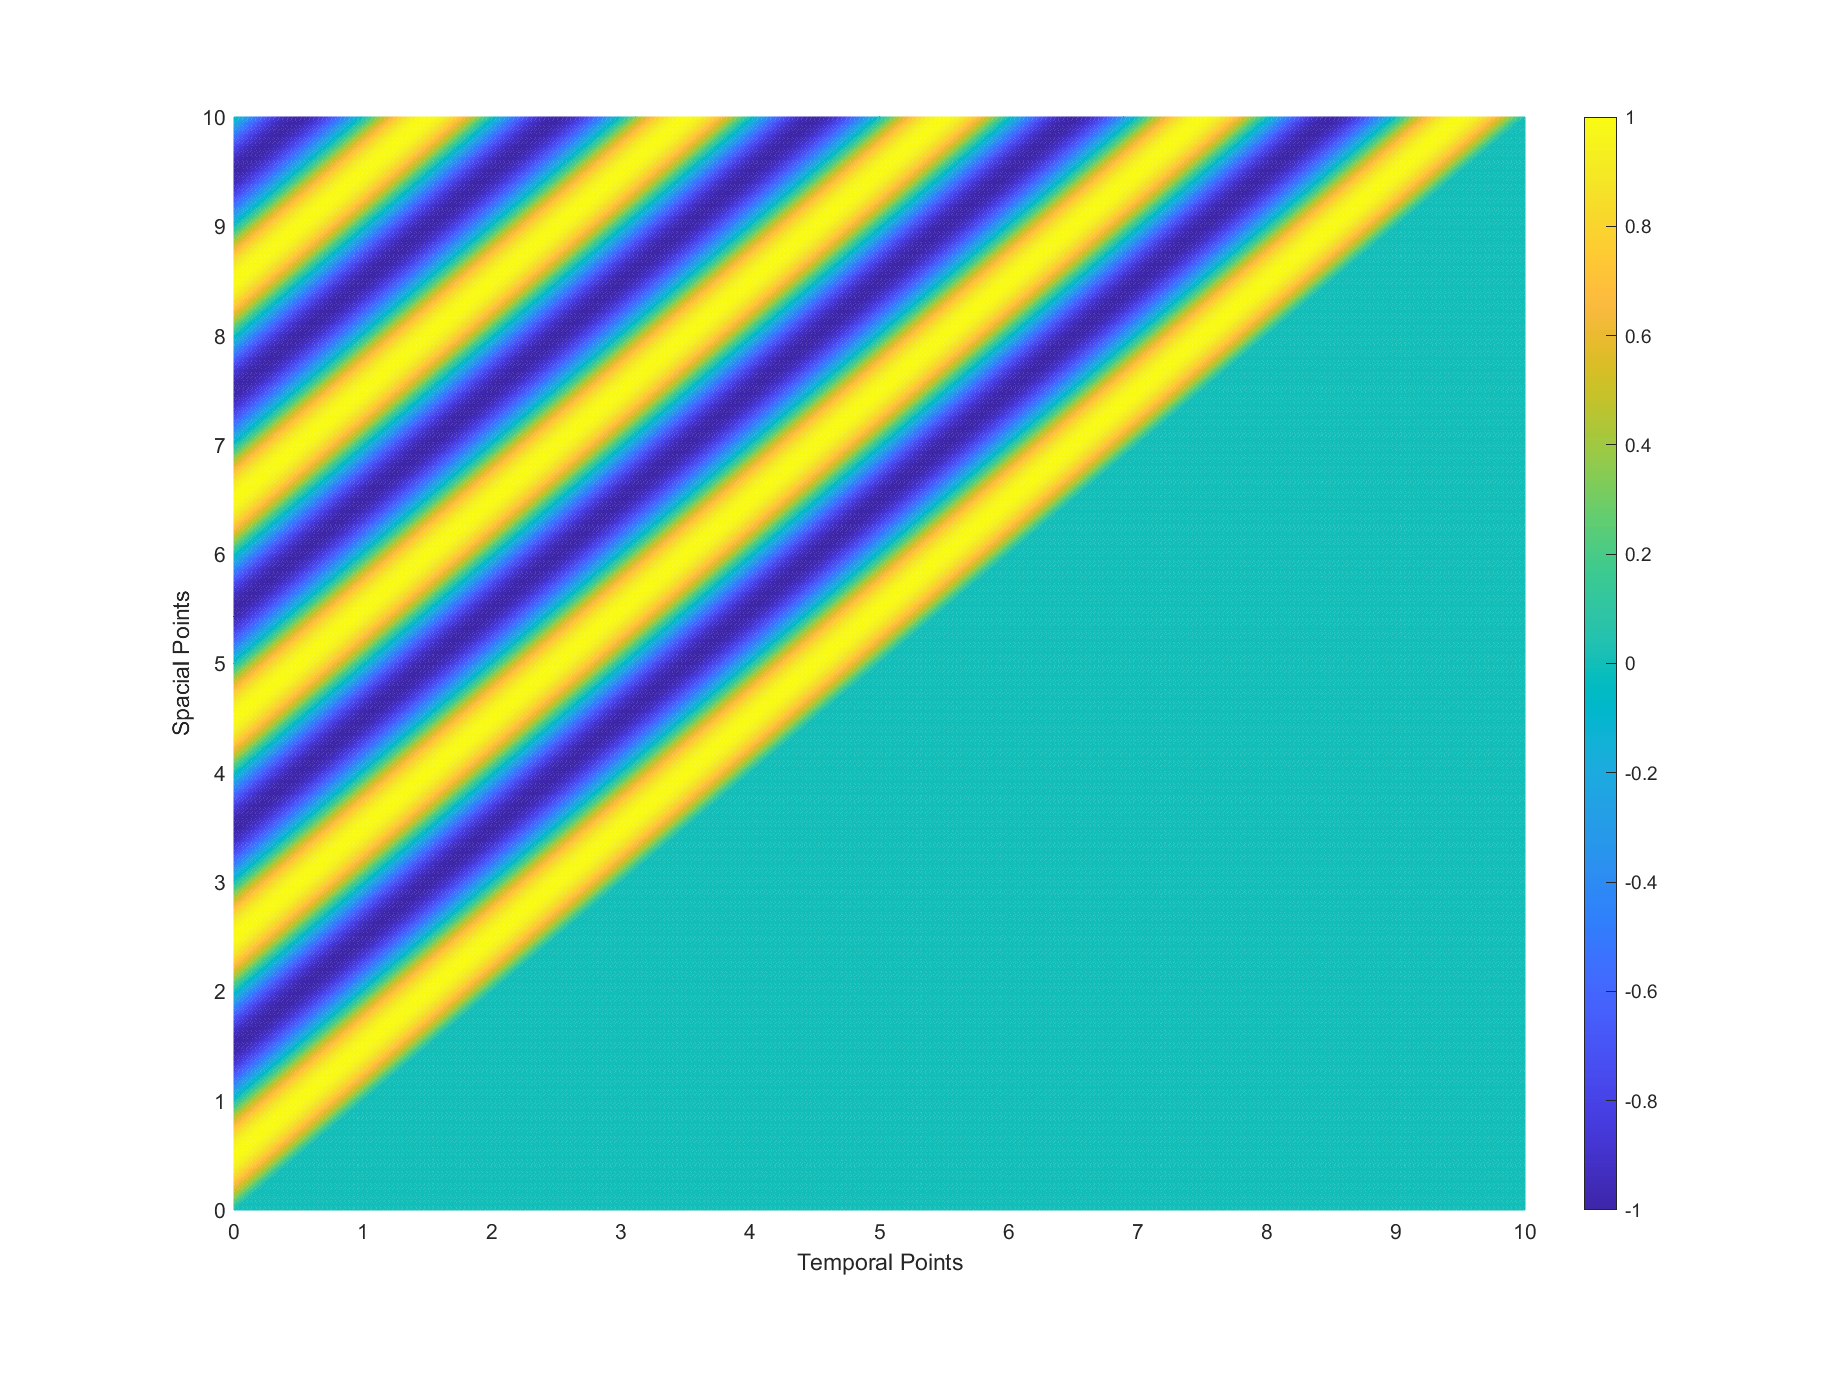
\includegraphics[width=\textwidth]{images/f0_top.eps}
			\caption{Top Down}
		\end{subfigure}
		\caption{Plots for \incode{f0} $= sin(\pi x)$.}
		\label{fig:both_images}
	\end{figure}

	\begin{figure}[htbp]
		\centering
		\begin{subfigure}[b]{0.45\textwidth}
			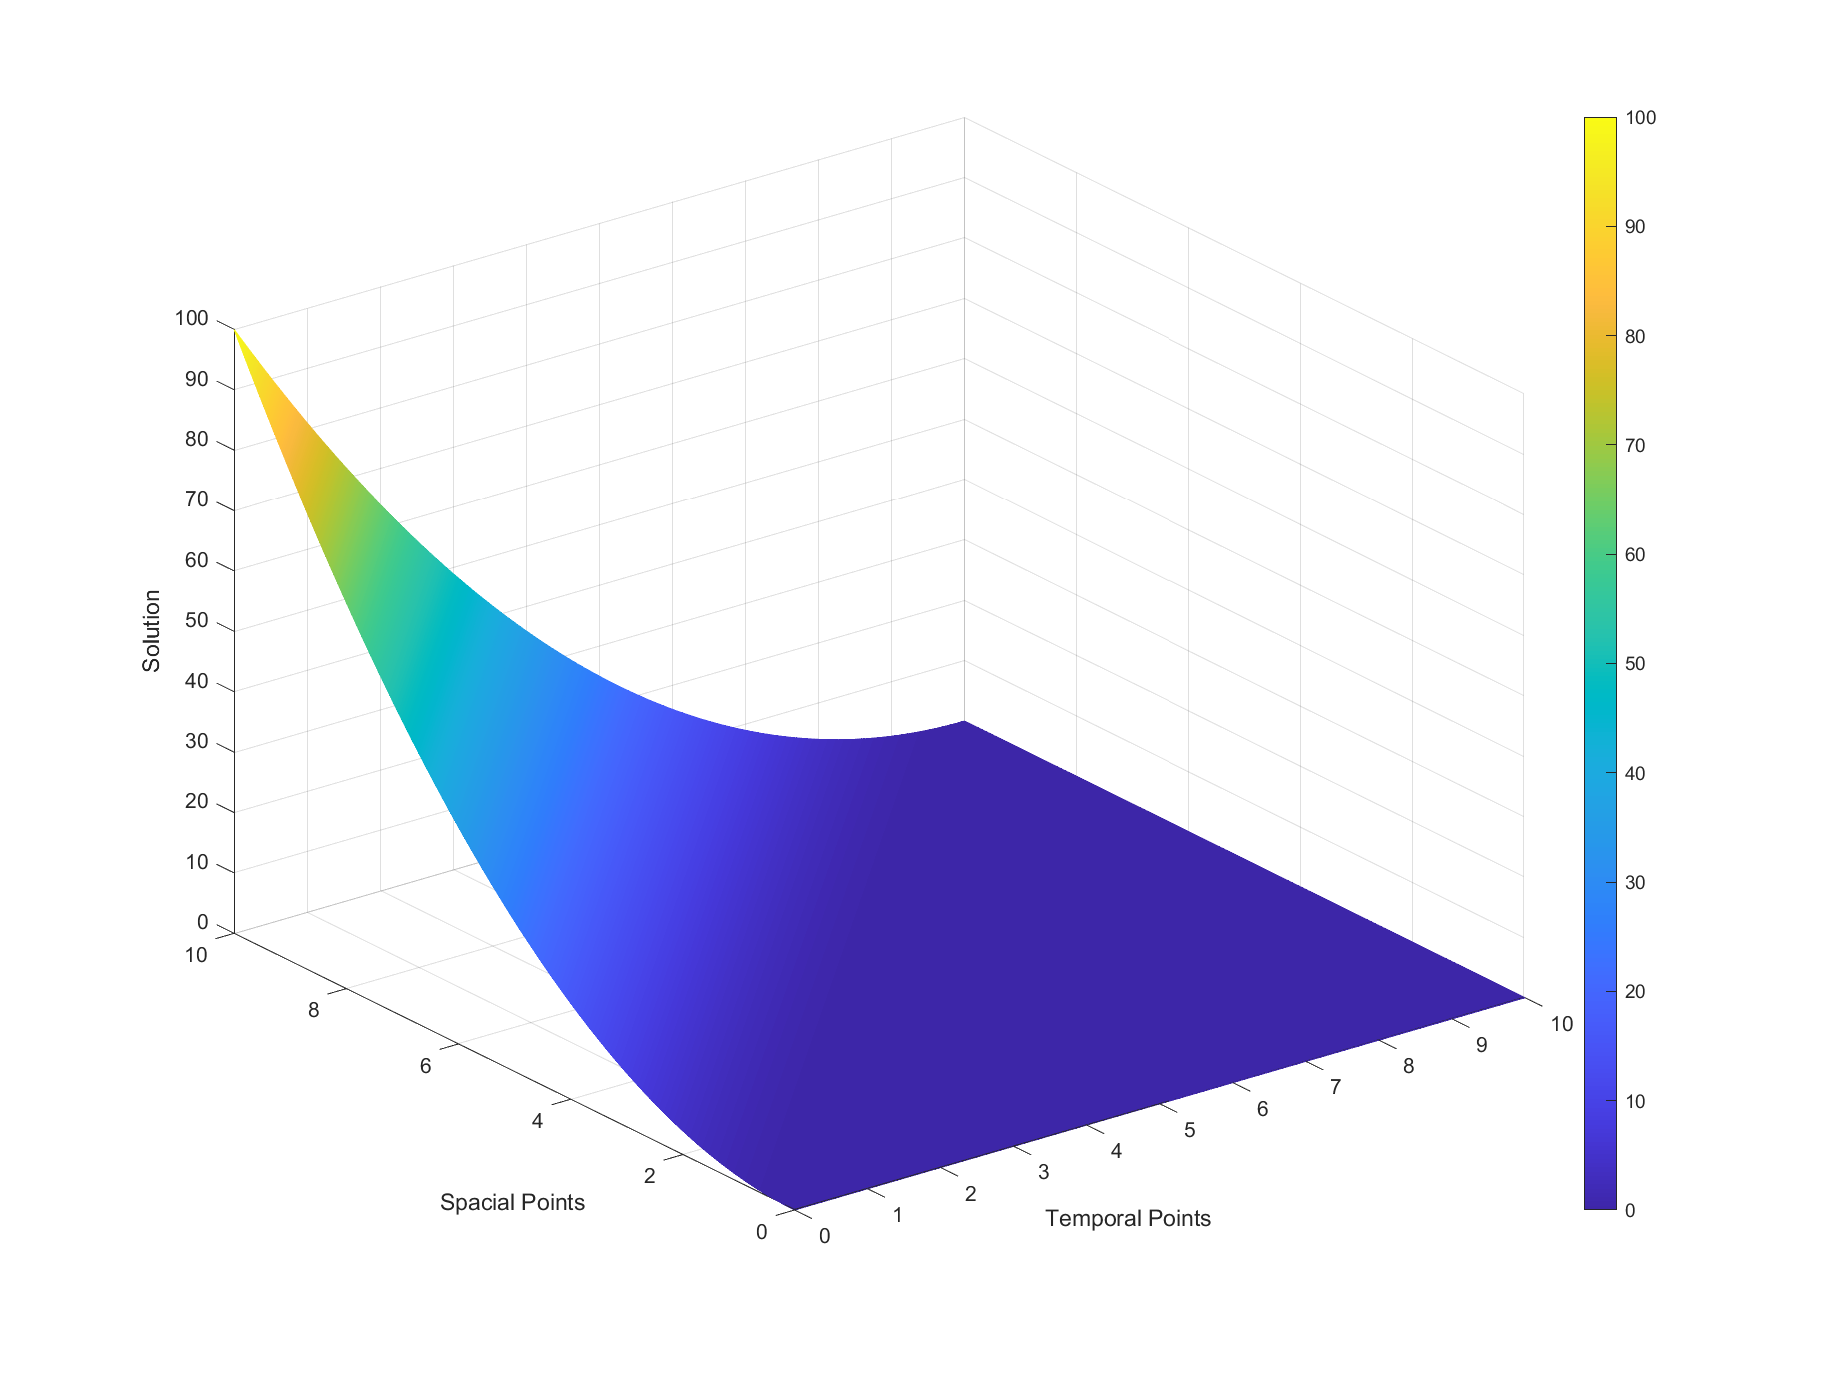
\includegraphics[width=\textwidth]{images/f1_side.eps}
			\caption{Side View}
		\end{subfigure}
		\hfill
		\begin{subfigure}[b]{0.45\textwidth}
			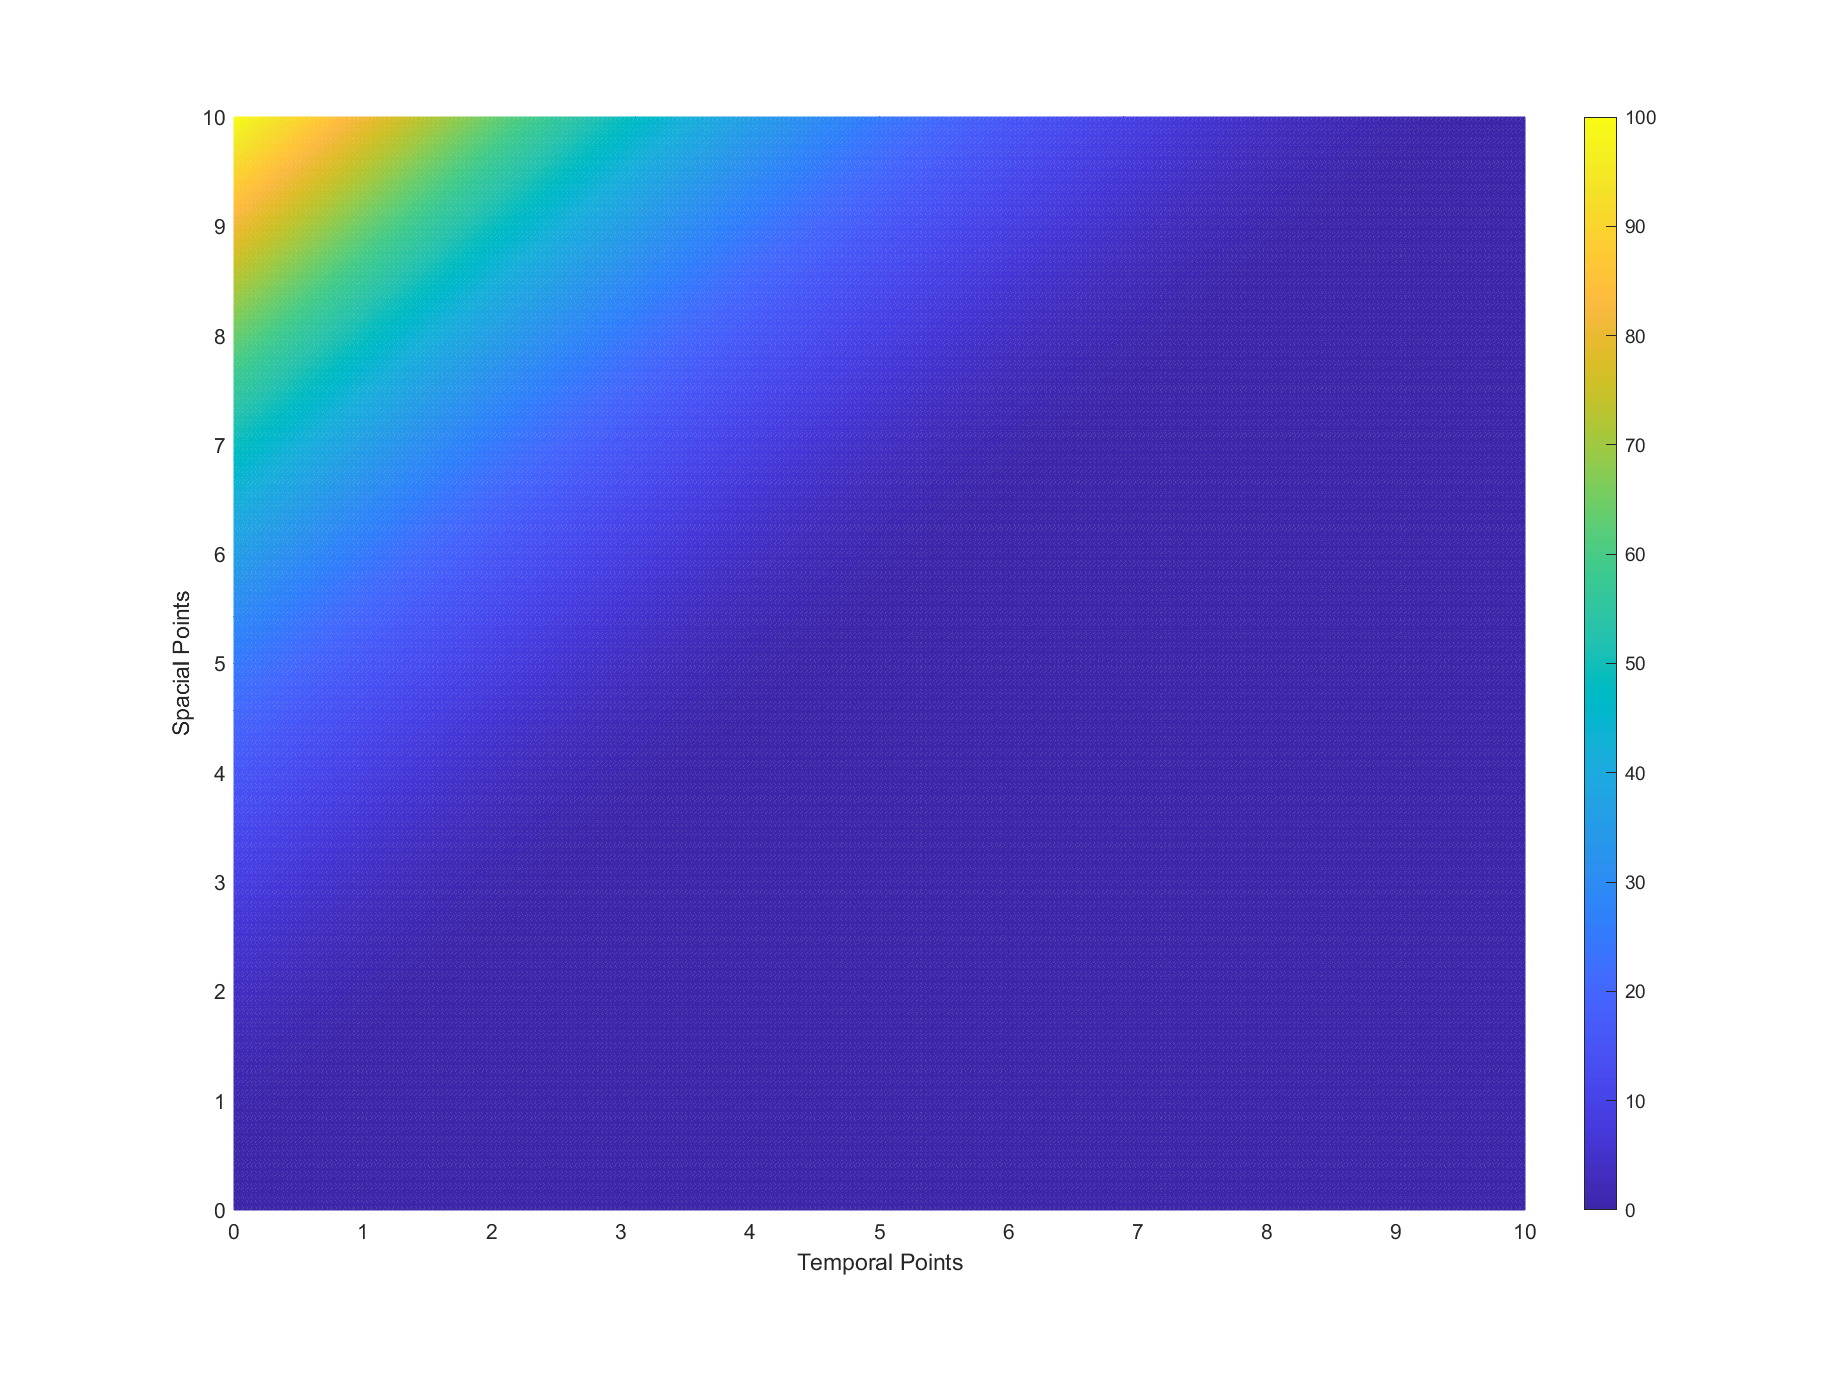
\includegraphics[width=\textwidth]{images/f1_top.eps}
			\caption{Top Down}
		\end{subfigure}
		\caption{Plots for \incode{f0} $= x^2$.}
		\label{fig:both_images}
	\end{figure}

	\begin{figure}[htbp]
		\centering
		\begin{subfigure}[b]{0.45\textwidth}
			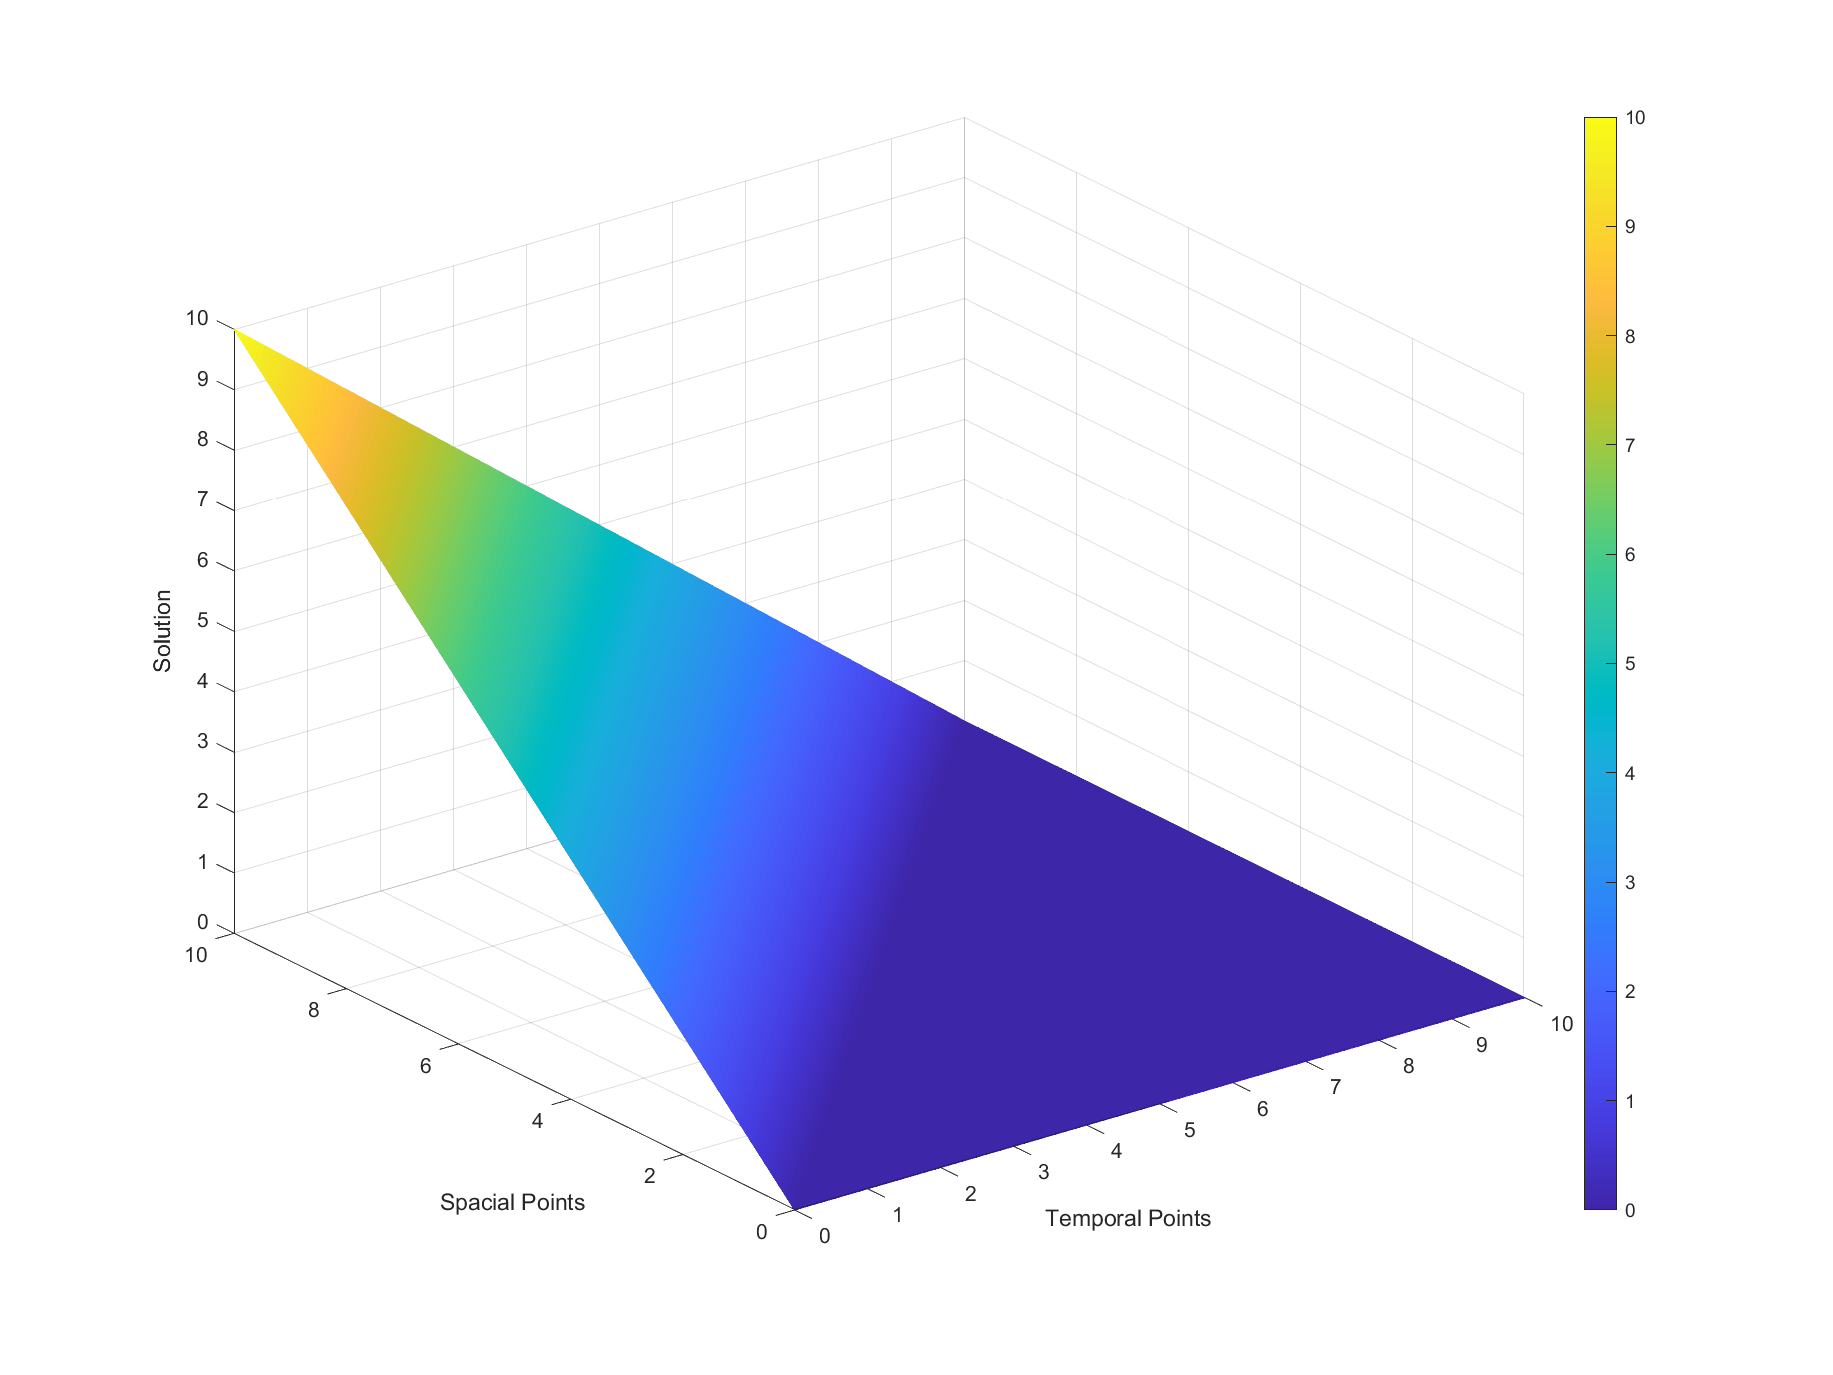
\includegraphics[width=\textwidth]{images/f2_side.eps}
			\caption{Side View}
		\end{subfigure}
		\hfill
		\begin{subfigure}[b]{0.45\textwidth}
			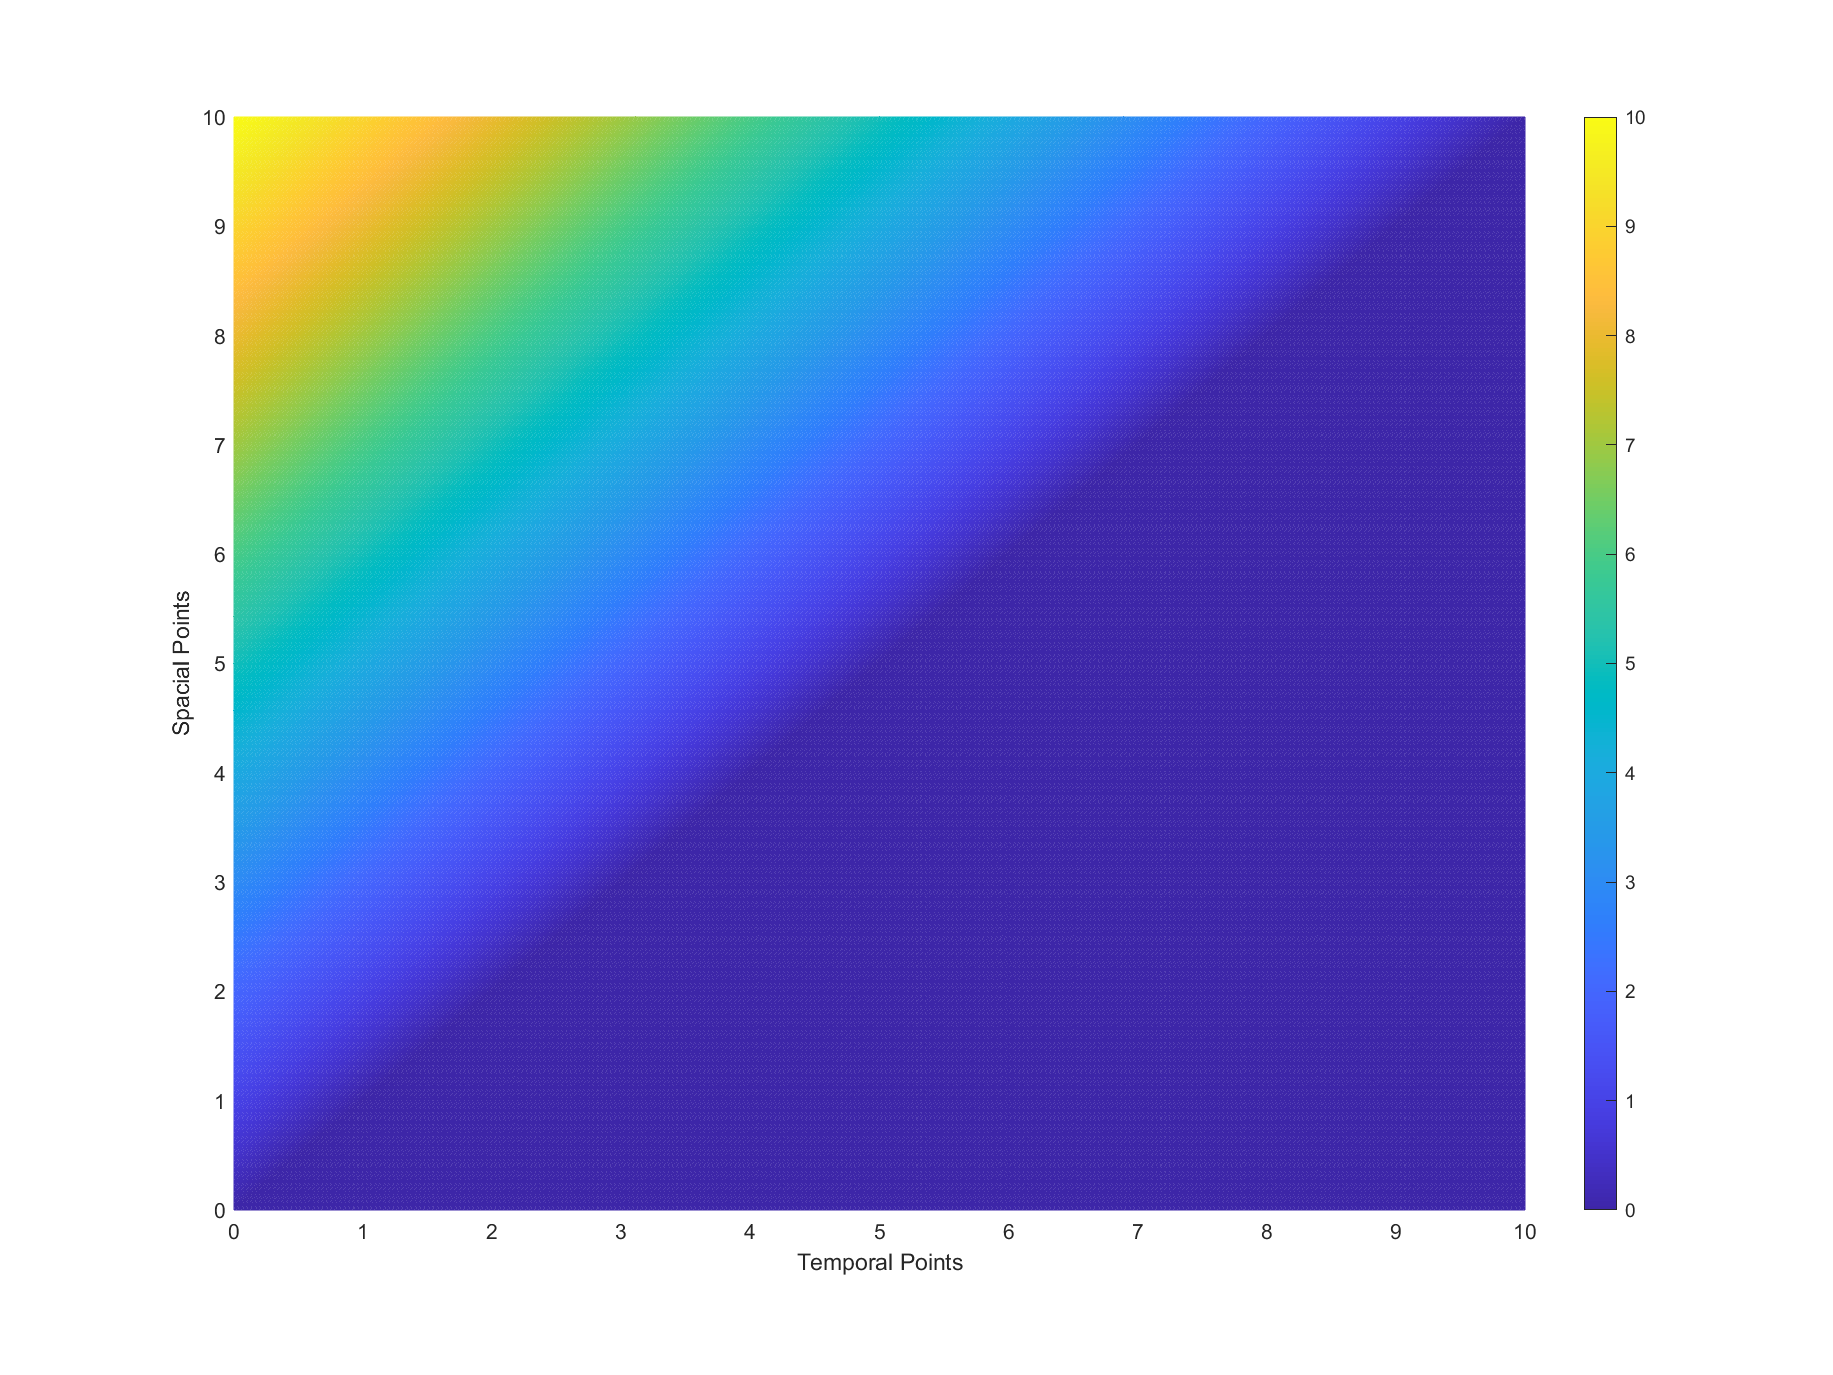
\includegraphics[width=\textwidth]{images/f2_top.eps}
			\caption{Top Down}
		\end{subfigure}
		\caption{Plots for \incode{f0} $= |x|$.}
		\label{fig:both_images}
	\end{figure}

	\subsection{Heat Equation}
	The heat equation is as follows:
	\begin{align}
		\frac{\partial u}{\partial t} = \frac{\partial^2 u}{\partial x^2} + \frac{\partial^2 u}{\partial y^2}
	\end{align}
	Below are some plots for the solutions to the heat equation. They were produced using \incode{main\_Heat2D.m}. The parameters used for the first set: \incode{dt} $= 0.01$, \incode{dx} $= 0.02$, \incode{dy} $= 0.02$, \incode{Tmax} $= 1$, \incode{Tsnap} $= [0.25, 0.5, 0.75, 1]$, \incode{value} $= 1$ and \incode{bounds} $= [0.3, 0.7, 0.3, 0.7]$. 
	
	\begin{figure}[htbp]
		\centering
		
		\begin{subfigure}[b]{0.45\textwidth}
			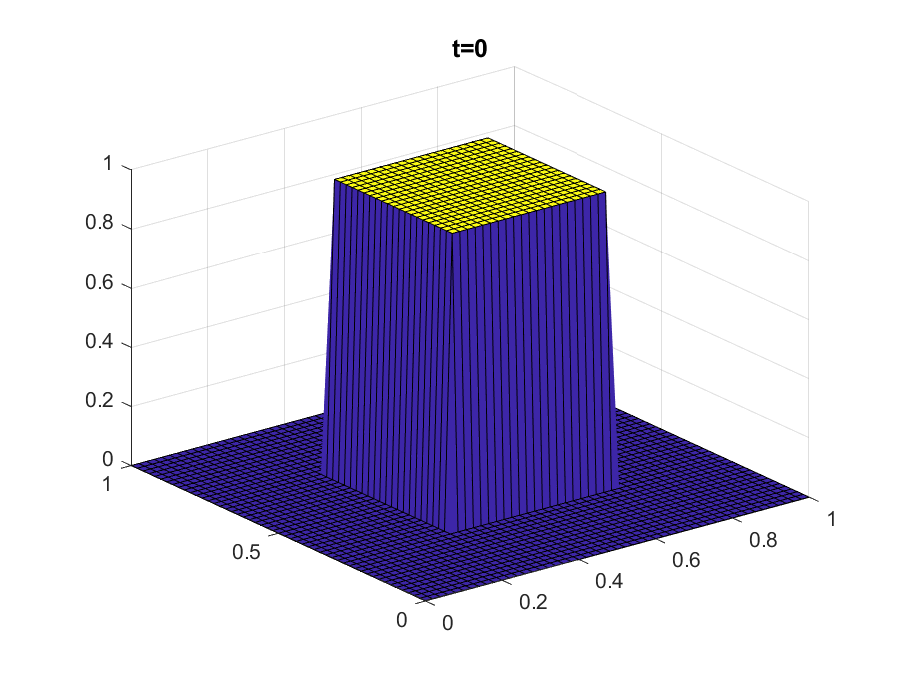
\includegraphics[width=\textwidth]{images/h1_t0.eps}
			\caption{$t = 0$}
			\label{fig:image1}
		\end{subfigure}
		\hfill
		\begin{subfigure}[b]{0.45\textwidth}
			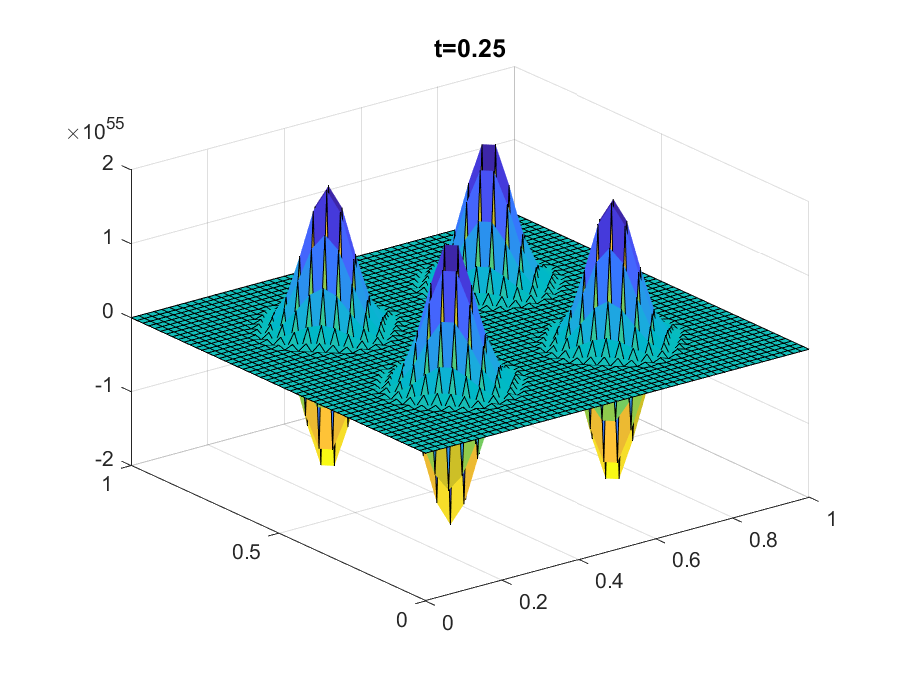
\includegraphics[width=\textwidth]{images/h1_t1.eps}
			\caption{$t = 0.25$}
			\label{fig:image2}
		\end{subfigure}
		
	\end{figure}
	\begin{figure}[htbp]
	\centering	
		\begin{subfigure}[b]{0.45\textwidth}
			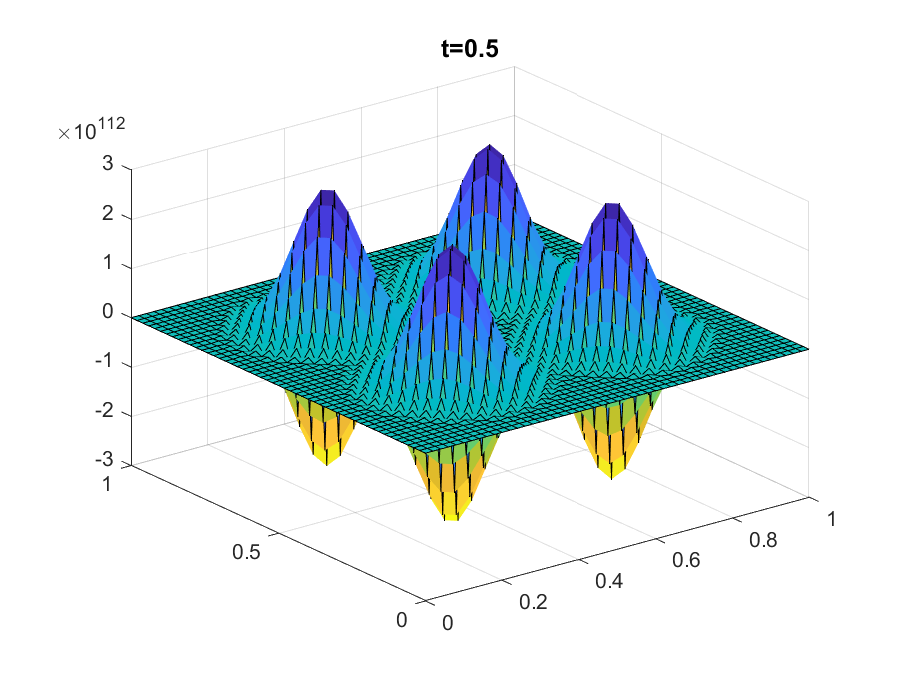
\includegraphics[width=\textwidth]{images/h1_t2.eps}
			\caption{$t = 0.5$}
			\label{fig:image4}
		\end{subfigure}
		\hfill
		\begin{subfigure}[b]{0.45\textwidth}
			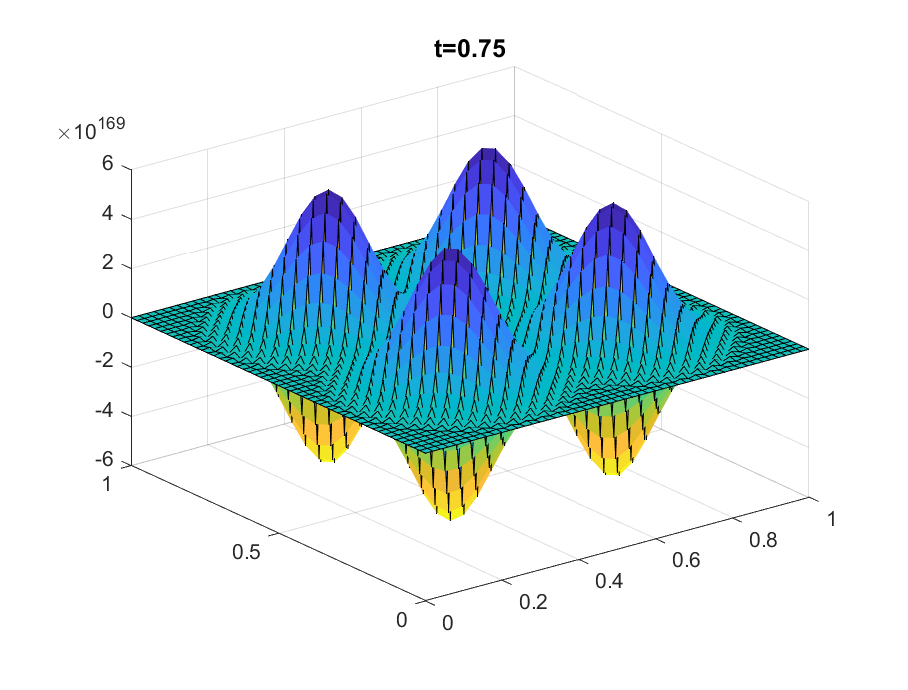
\includegraphics[width=\textwidth]{images/h1_t3.eps}
			\caption{$t = 0.75$}
			\label{fig:image5}
		\end{subfigure}
		\end{figure}
	\begin{figure}[htbp]
	\centering	
		\vspace{1em}
		
		\begin{subfigure}[b]{0.45\textwidth}
			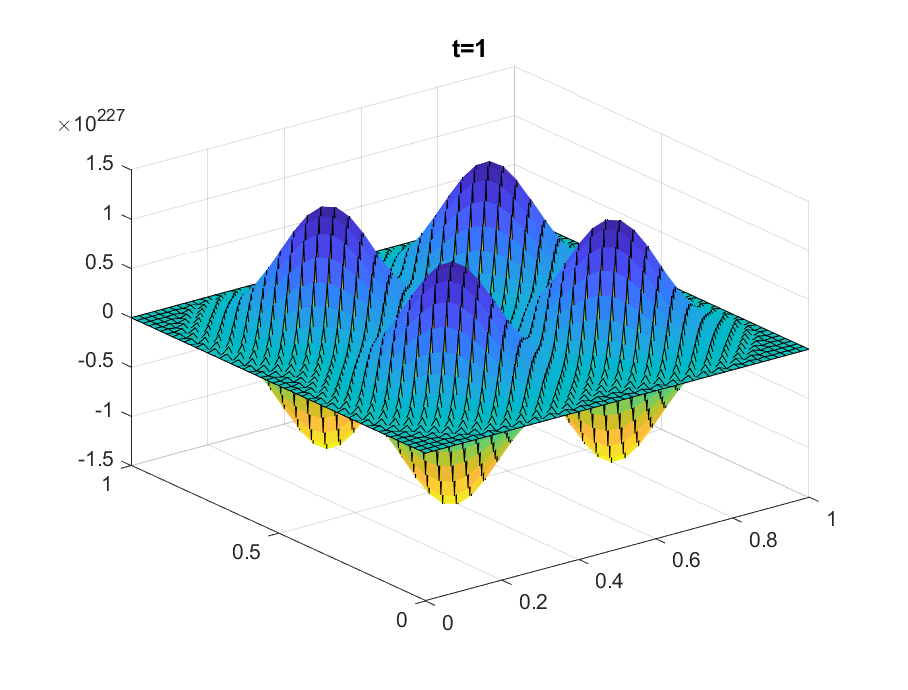
\includegraphics[width=\textwidth]{images/h1_t4.eps}
			\caption{$t = 1$}
			\label{fig:image7}
		\end{subfigure}


		\label{fig:all_images}
	\end{figure}
	\newpage 
	The parameters used for the second set: \incode{dt} $= 0.01$, \incode{dx} $= 0.02$, \incode{dy} $= 0.02$, \incode{Tmax} $= 1$, \incode{Tsnap} $= [0.25, 0.5, 0.75, 1]$, \incode{value} $= 1$ and \incode{bounds} $= [0.3, 0.7, 0.3, 0.7]$. 
	
	\begin{figure}[htbp]
		\centering
		
		\begin{subfigure}[b]{0.45\textwidth}
			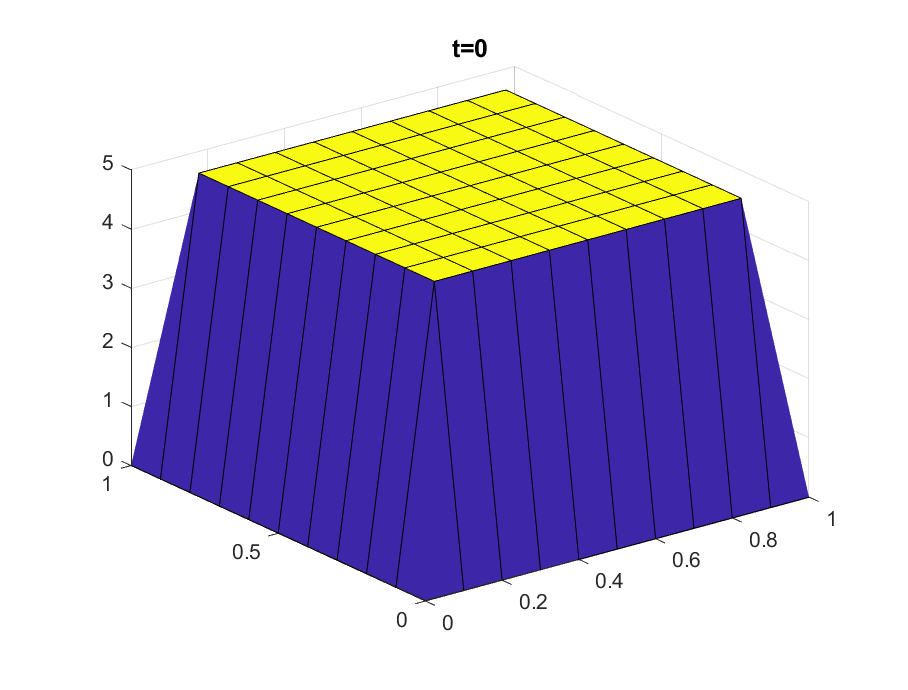
\includegraphics[width=\textwidth]{images/h2_t0.eps}
			\caption{$t = 0$}
			\label{fig:image1}
		\end{subfigure}
		\hfill
		\begin{subfigure}[b]{0.45\textwidth}
			\includegraphics[width=\textwidth]{images/h2_t1.eps}
			\caption{$t = 1$}
			\label{fig:image2}
		\end{subfigure}
		
	\end{figure}
	\begin{figure}[htbp]
		\centering	
		\begin{subfigure}[b]{0.45\textwidth}
			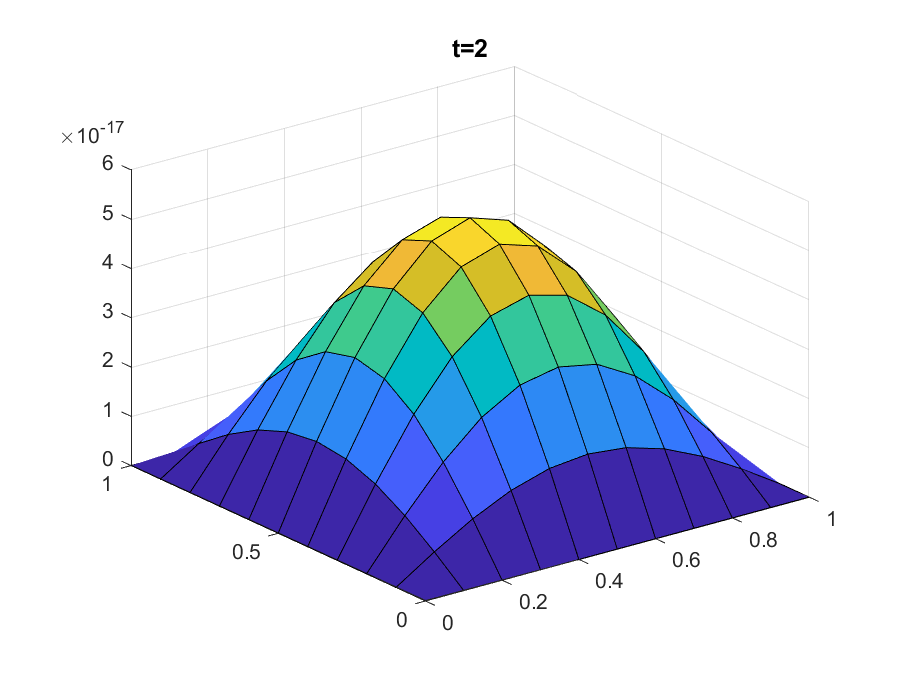
\includegraphics[width=\textwidth]{images/h2_t2.eps}
			\caption{$t = 2$}
			\label{fig:image4}
		\end{subfigure}
		\hfill
		\begin{subfigure}[b]{0.45\textwidth}
			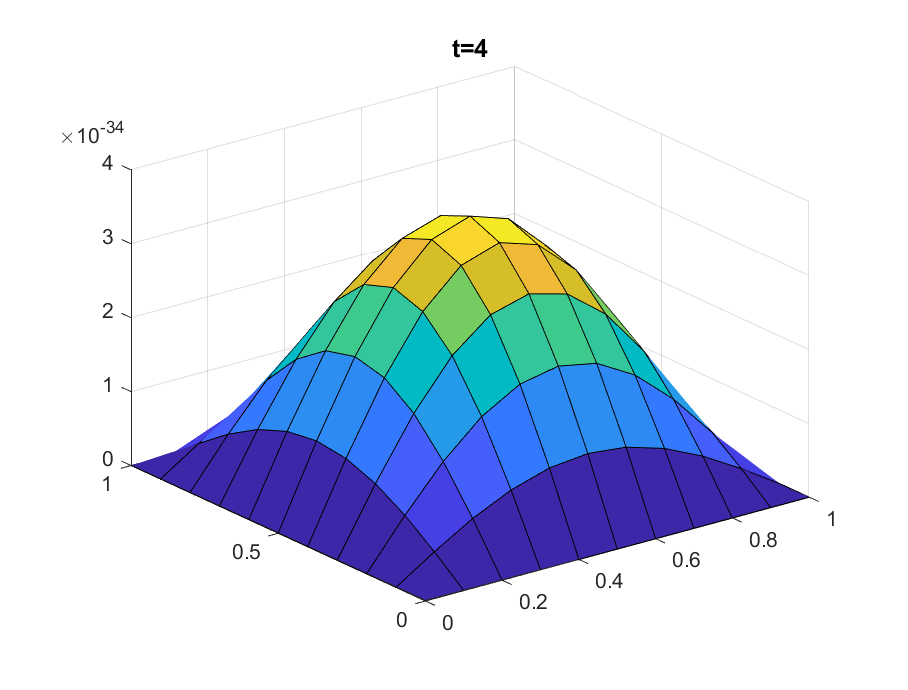
\includegraphics[width=\textwidth]{images/h2_t3.eps}
			\caption{$t = 4$}
			\label{fig:image5}
		\end{subfigure}
	\end{figure}
	\begin{figure}[htbp]
		\centering	
		\vspace{1em}
		
		\begin{subfigure}[b]{0.45\textwidth}
			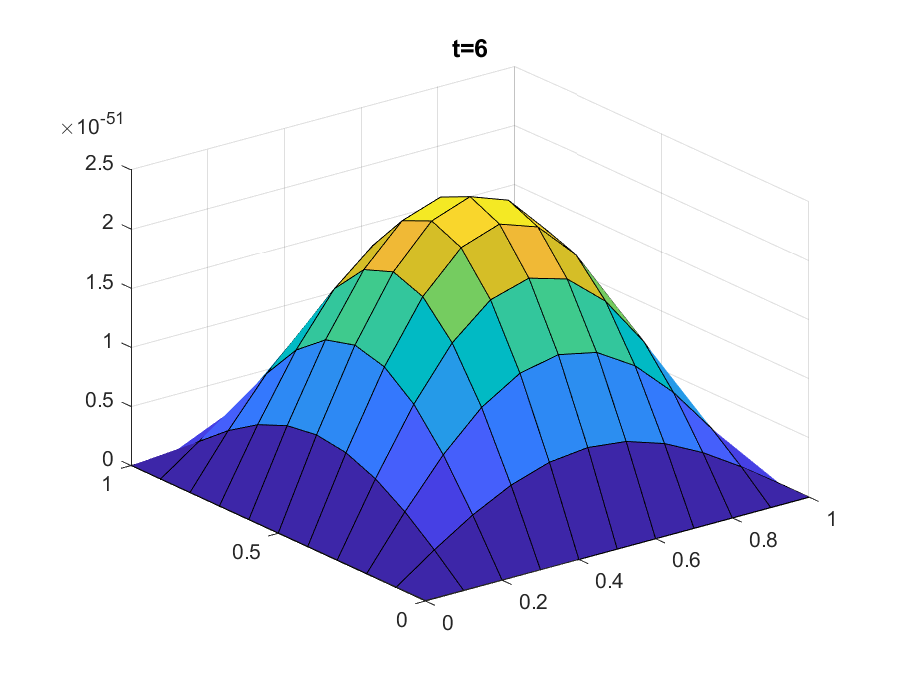
\includegraphics[width=\textwidth]{images/h2_t4.eps}
			\caption{$t = 6$}
			\label{fig:image7}
		\end{subfigure}
	\hfill
			\begin{subfigure}[b]{0.45\textwidth}
		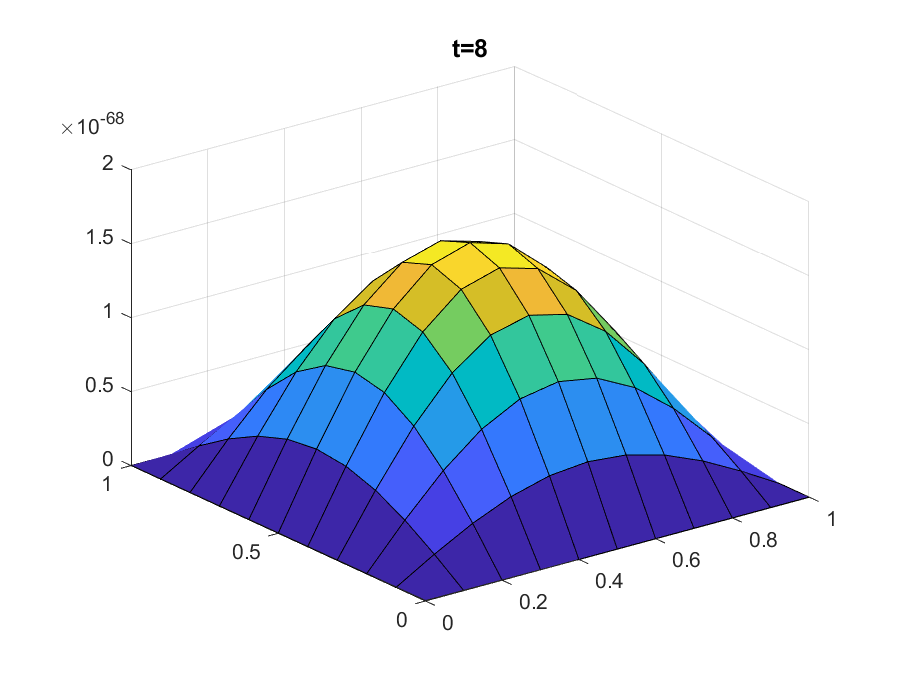
\includegraphics[width=\textwidth]{images/h2_t5.eps}
		\caption{$t = 8$}
		\label{fig:image4}
	\end{subfigure}

		\label{fig:all_images}
	\end{figure}
	\begin{figure}[htbp]
		\centering	
		\begin{subfigure}[b]{0.45\textwidth}
			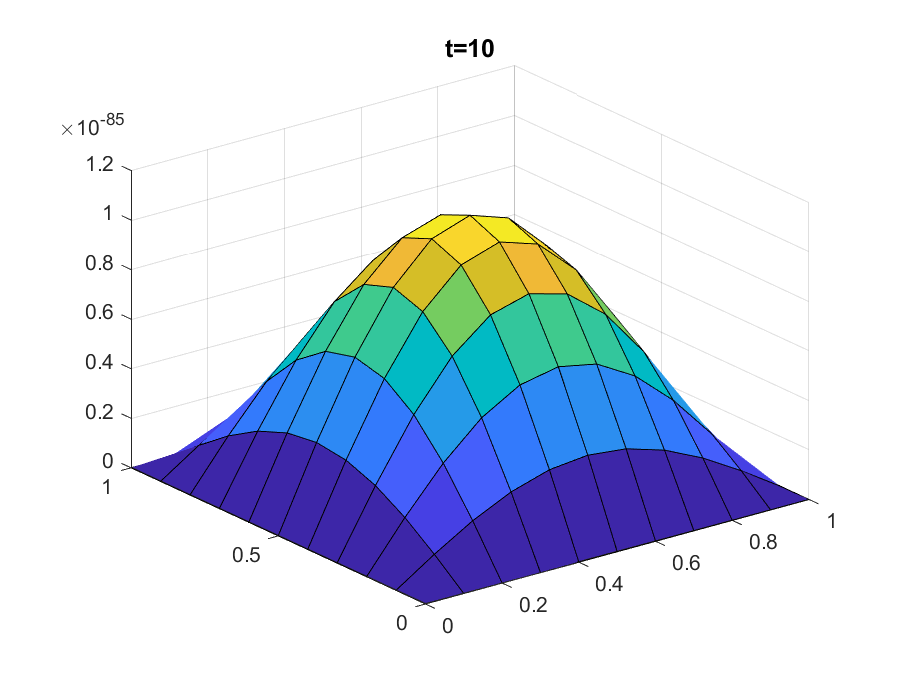
\includegraphics[width=\textwidth]{images/h2_t6.eps}
			\caption{$t = 10$}
			\label{fig:image5}
		\end{subfigure}
	\end{figure}
	\newpage
	in \incode{ModHeat2D.m}, we've modified the original code and added a parameter \incode{alpha}. A heat sink has been placed at coordinate $(0.25, 0.25)$. The strength of this sink is represented by the parameter \incode{alpha} with a higher value leading to a greater reduction in heat at that location. I've used the same parameters from the second set of images and taken alpha to be positive and negative. You can see in the following plots that the sink has a dramatic effect on the heat distribution over time. 
	
	\begin{figure}[htbp]
		\centering	
		\begin{subfigure}[b]{0.45\textwidth}
			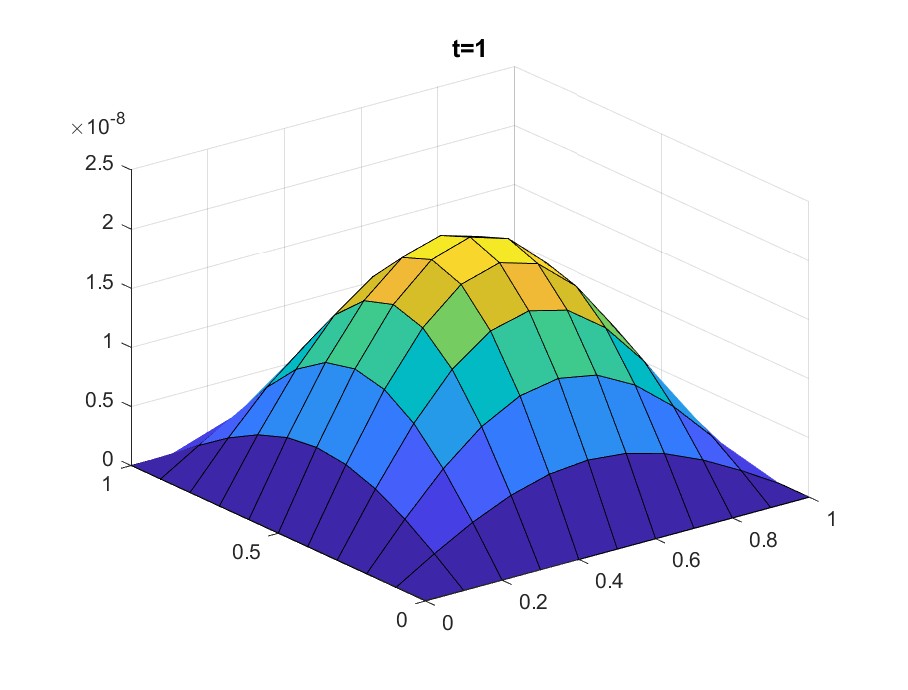
\includegraphics[width=\textwidth]{images/h3_t1.eps}
			\caption{$t = 1$}
			\label{fig:image4}
		\end{subfigure}
		\hfill
		\begin{subfigure}[b]{0.45\textwidth}
			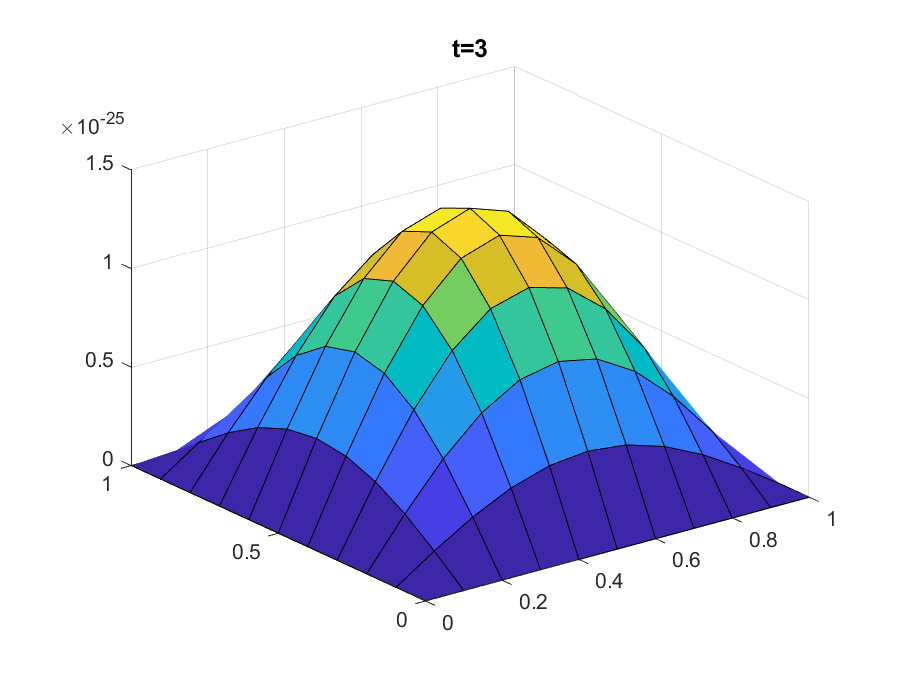
\includegraphics[width=\textwidth]{images/h3_t2.eps}
			\caption{$t = 3$}
			\label{fig:image5}
		\end{subfigure}
	\end{figure}
	\begin{figure}[htbp]
		\centering	
		\vspace{1em}
		
		\begin{subfigure}[b]{0.45\textwidth}
			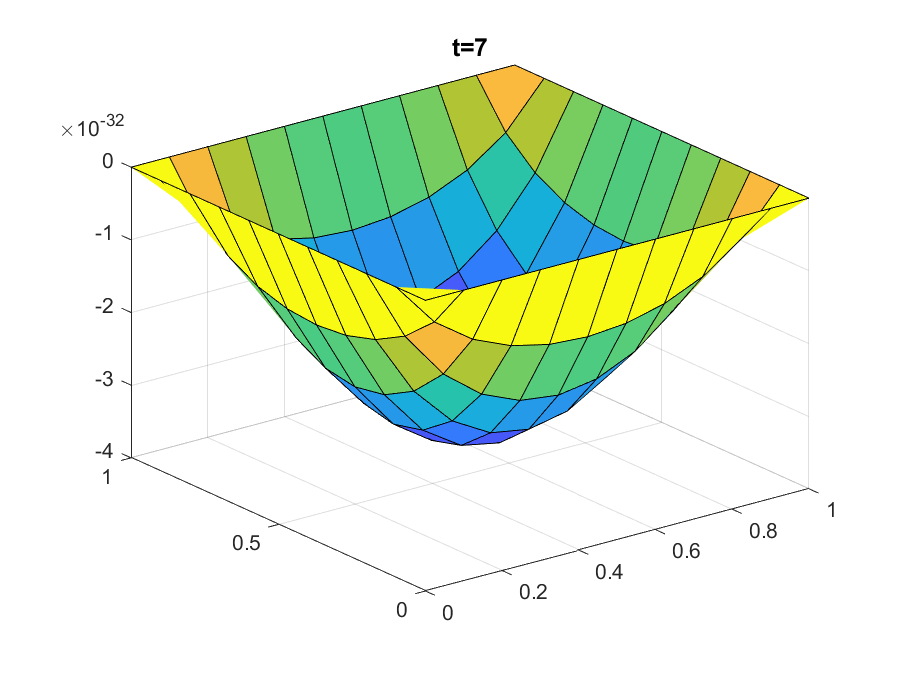
\includegraphics[width=\textwidth]{images/h3_t3.eps}
			\caption{$t = 7$}
			\label{fig:image7}
		\end{subfigure}
		\hfill
		\begin{subfigure}[b]{0.45\textwidth}
			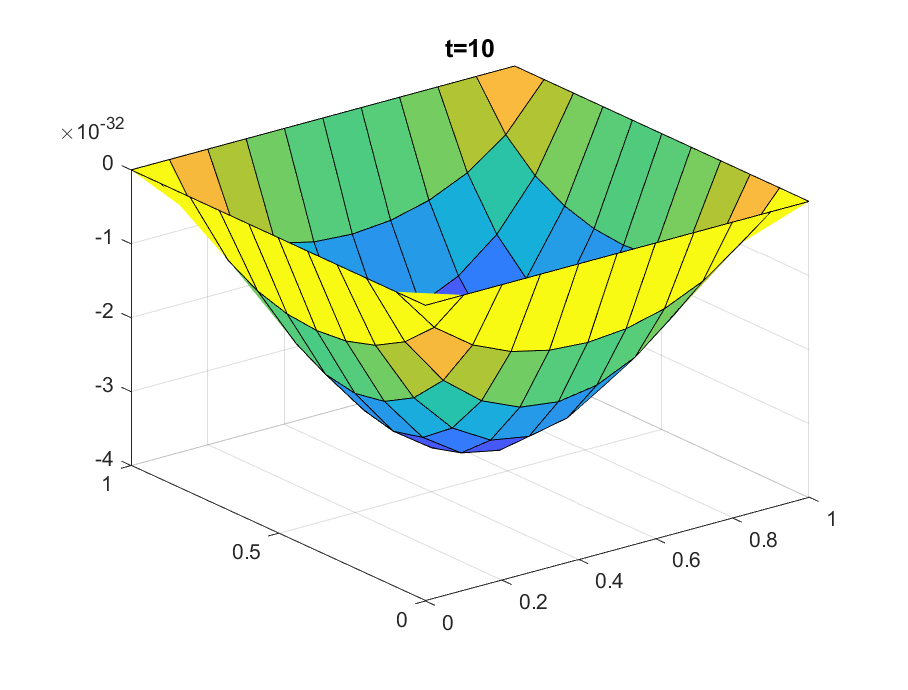
\includegraphics[width=\textwidth]{images/h3_t4.eps}
			\caption{$t = 10$}
			\label{fig:image4}
		\end{subfigure}
		
		\caption{Negative value for alpha ($\alpha = 5 \times 10^{-34}$).}
		\label{fig:all_images}
	\end{figure}
	\newpage
	When we give it a negative value, it becomes a heat source rather than a sink. This leads to similar qualitative behaviour as in the original code but the reduction in heat is slower. 
	
	\begin{figure}[htbp]
		\centering	
		\begin{subfigure}[b]{0.45\textwidth}
			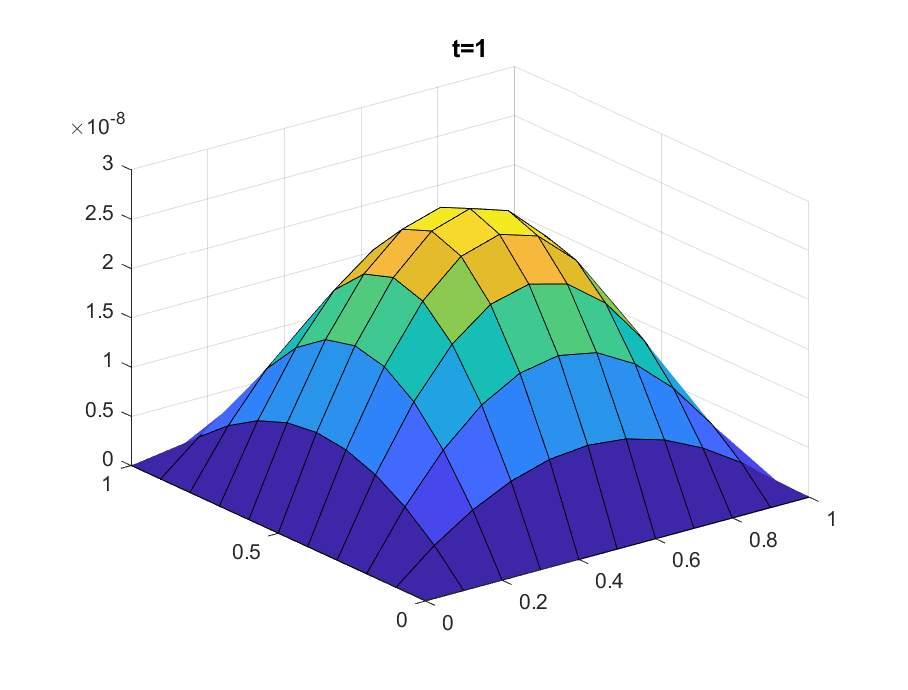
\includegraphics[width=\textwidth]{images/h4_t1.eps}
			\caption{$t = 1$}
			\label{fig:image4}
		\end{subfigure}
		\hfill
		\begin{subfigure}[b]{0.45\textwidth}
			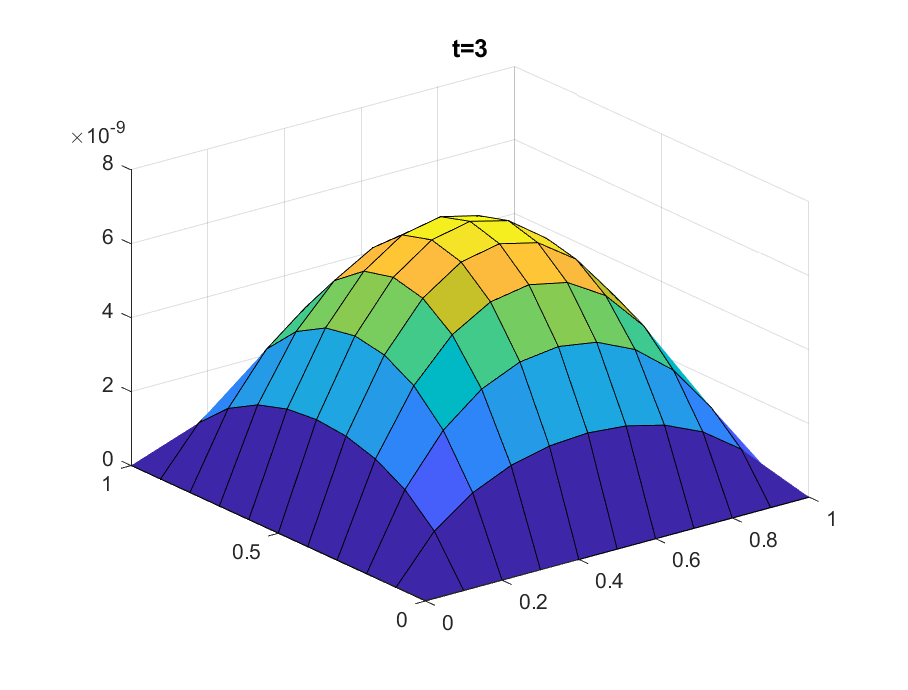
\includegraphics[width=\textwidth]{images/h4_t2.eps}
			\caption{$t = 3$}
			\label{fig:image5}
		\end{subfigure}
	\end{figure}
	\begin{figure}[htbp]
		\centering	
		\vspace{1em}
		
		\begin{subfigure}[b]{0.45\textwidth}
			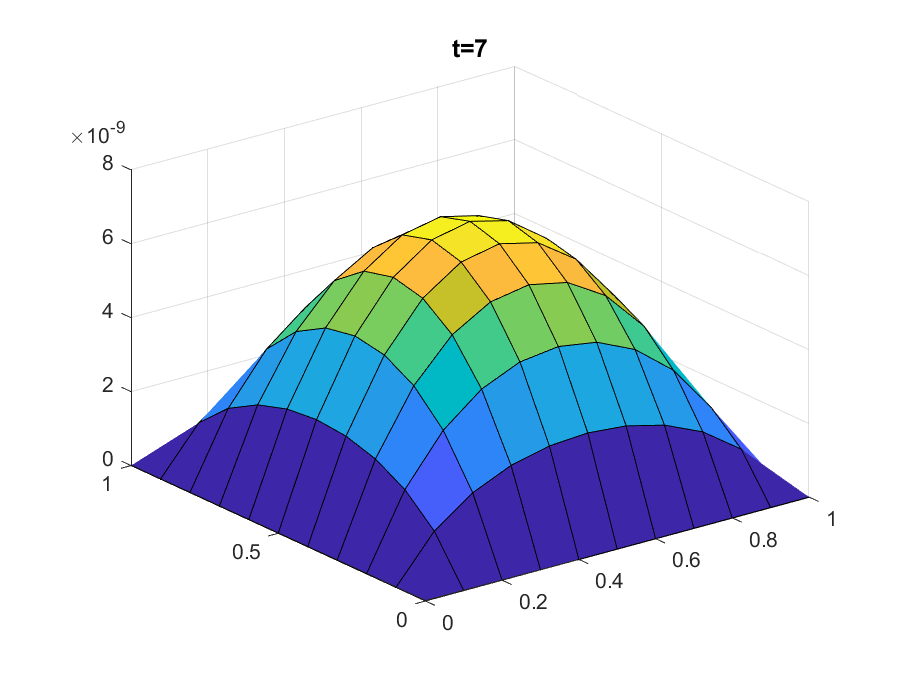
\includegraphics[width=\textwidth]{images/h4_t3.eps}
			\caption{$t = 7$}
			\label{fig:image7}
		\end{subfigure}
		\hfill
		\begin{subfigure}[b]{0.45\textwidth}
			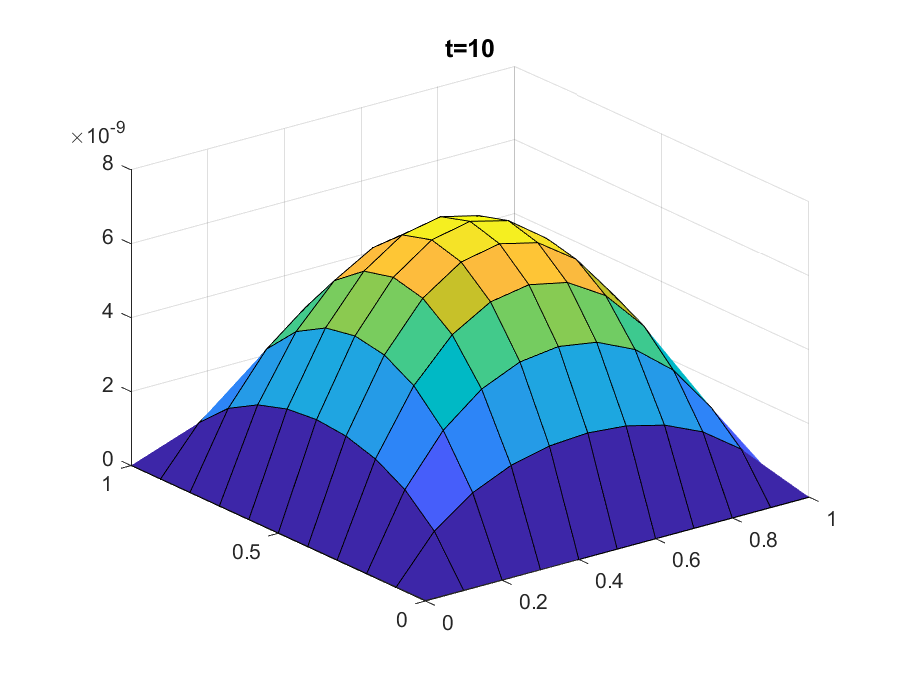
\includegraphics[width=\textwidth]{images/h4_t4.eps}
			\caption{$t = 10$}
			\label{fig:image4}
		\end{subfigure}
		
		\caption{Negative value for alpha ($\alpha = -1 \times 10^{-10}$).}
		\label{fig:all_images}
	\end{figure}
	\newpage
	\section{Stage 3}
	This section is concerned with the Insect Dispersal Model:
	\begin{align}
		n_t &= d_0 \left( \left(\frac{n}{n_0}\right)^m n_x \right)_x 
	\end{align}
	We first need to simplify the equation to make it easier to discretise:
	\begin{align}
		n_t &= d_0 \left( \left(\frac{n}{n_0}\right)^m n_x \right)_x \\
		&= \frac{d}{n_{0}^m} \left( n^m n_x \right)_x \\
		&= \frac{d}{n_{0}^m} \left( mn^{n - 1} (n_x)^2 + n^m n_{xx} \right) \\
		&= \frac{dn^{m - 1}}{n_{0}^m} \left( m(n_x)^2 + nn_{xx} \right) 
	\end{align}
	We will define each partial derivative:
	\begin{align}
		n_{xx} &\approx \frac{n_{i + 1, j} + n_{i - 1, j} -2n_{i, j}}{(\Delta x)^2} \\
		n_x &\approx \frac{n_{i + 1, j} - n_{i - 1, j}}{2(\Delta x)} \\
		n_t &\approx \frac{n_{i, j + 1} - n_{i, j}}{\Delta t} 
	\end{align}
	We can use a couple of facts about the behaviour of our system at certain points to simplify:
	\begin{align}
		n_x&(-x, t) = n_x(x, t) = 0 \\ n_x &= 0 \\ n(0, 0) &= 0
	\end{align}
	And then substitute and simplify:
	\begin{align}
		n_{i, j + 1} = n_{i,j} + \frac{d_0 n_{i, j}^{m - 1} \Delta t}{n_0^m} \left( n_{i,j} \frac{n_{i + 1, j} + n_{i - 1, j} - 2n_{i, j}}{(\Delta x)^2} \right)
	\end{align}
	You can find an implementation of this in \incode{dispersal.m} which can be run from \incode{main\_dispersal.m}. The parameters used to generate the following plots: \incode{xmin} $= -10$, \incode{dx} $= 0.1$, \incode{xmax} $= 10$, \incode{dt} $= 0.001$, \incode{tmax} $= 50$, \incode{d0} $= 0.5$, \incode{m} $= 0.5$, \incode{n0} $= 150$ and \incode{Q} $= 100$. 
	
	You can find the MATLAB implementation in \incode{dispersal.m}. To view the results, run \incode{main\_dispersal.m}. The following graph was produced using the following parameters: \incode{xmin} $= 0$, \incode{dx} $= 0.1$, \incode{xmax} $= 20$, \incode{dt} $= 0.001$, \incode{tmax} $= 50$, \incode{d0} $= 1.5$, \incode{m} $= 0.5$, \incode{n0} $= 150$ and \incode{Q} $= 100$. 
	
	\begin{figure}[h]
		\centering
		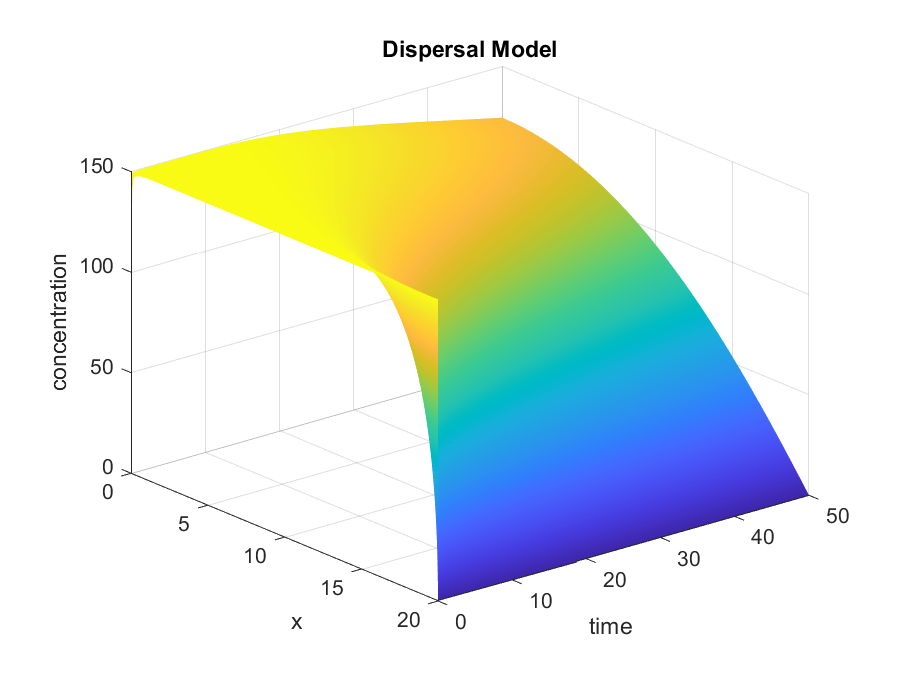
\includegraphics[width = 0.75\textwidth]{images/dispersal.eps}
		\caption{Graph of insect density distribution across time.}
	\end{figure}
	\newpage
	When considering how to add a wind factor, we need to determine what the effect of the wind will be. We will presume that the wind component $wn_x$ will directly influence the population density such that the new form of the equation will be:
	\begin{align}
		n_t &= d_0 \left( \left( \left(\frac{n}{n_0}\right)^m + w \right) n_x \right)_x 
	\end{align}
	If included in this way, a positive value for $w$ would increase the rate of change of the population density with respect to time. A negative value would have the opposite effect, decreasing the rate of change.  
\end{document}          
